\subsection{Preliminary results}

% ----------------------------------- Orange -----------------------------------
\subsubsection{Image \texttt{orange}. Varying $\sigma_s^2$.}

\noindent\makebox[\textwidth][c]{%
\begin{minipage}{\linewidth}
  \begin{minipage}{0.45\linewidth}
    \begin{figure}[H]
      \centering
      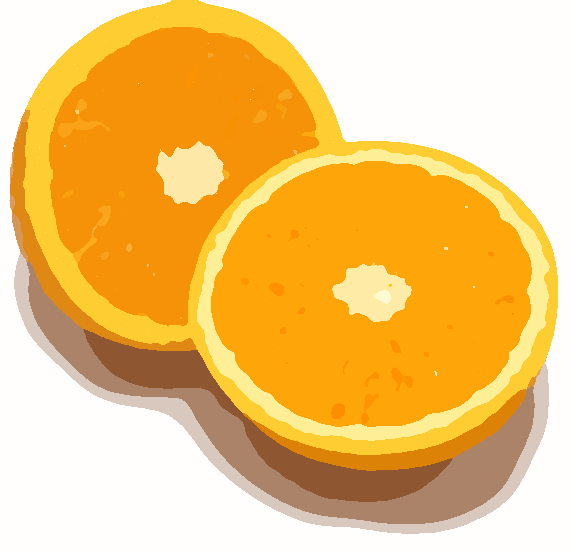
\includegraphics[scale=0.4]{./images/02/orange/meanshift1_3_4.png}
      \caption{Image \texttt{orange} segmented with \texttt{mean-shift}.
        $(\sigma_s^2, \sigma_c^2) \equiv (3.0, 4.0)$}
      \label{fig:02_orange1_3_4}
    \end{figure}
  \end{minipage}
  \hfill
  \begin{minipage}{0.45\linewidth}
    \begin{figure}[H]
      \centering
      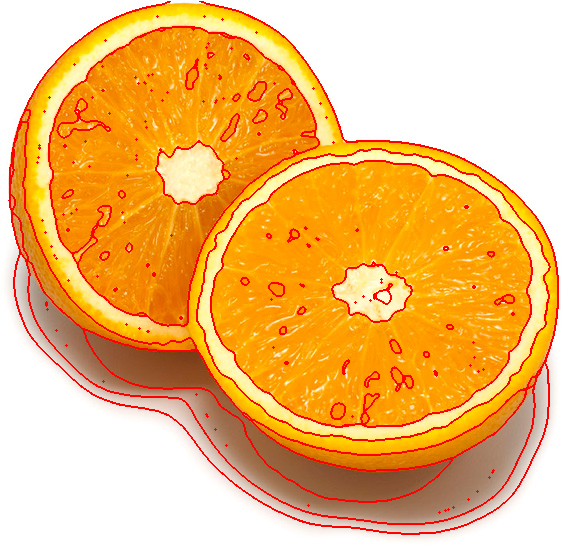
\includegraphics[scale=0.4]{./images/02/orange/meanshift2_3_4.png}
      \caption{Segmentation bounds of image \texttt{orange}.
        $(\sigma_s^2, \sigma_c^2) \equiv (3.0, 4.0)$}
      \label{fig:02_orange2_3_4}
    \end{figure}
  \end{minipage}
\end{minipage}
}

\noindent\makebox[\textwidth][c]{%
\begin{minipage}{\linewidth}
  \begin{minipage}{0.45\linewidth}
    \begin{figure}[H]
      \centering
      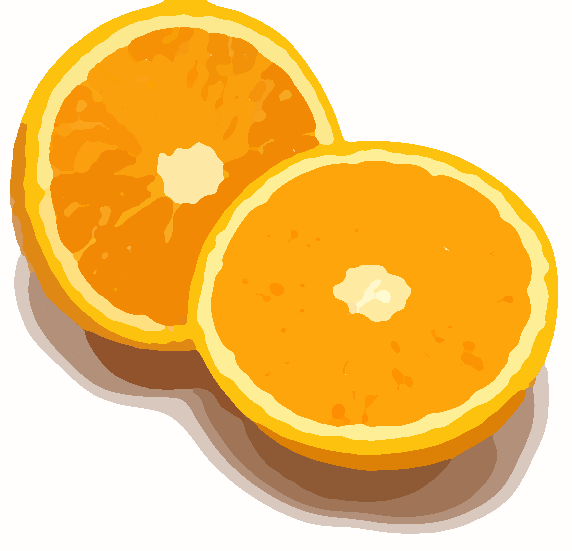
\includegraphics[scale=0.4]{./images/02/orange/meanshift1_4_4.png}
      \caption{Image \texttt{orange} segmented with \texttt{mean-shift}.
        $(\sigma_s^2, \sigma_c^2) \equiv (4.0, 4.0)$}
      \label{fig:02_orange1_4_4}
    \end{figure}
  \end{minipage}
  \hfill
  \begin{minipage}{0.45\linewidth}
    \begin{figure}[H]
      \centering
      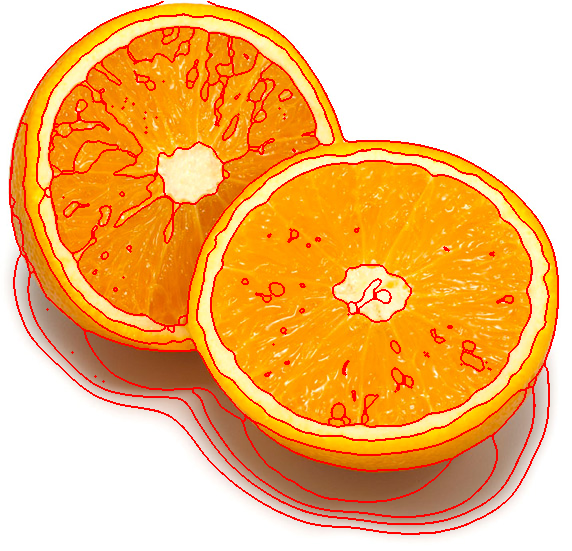
\includegraphics[scale=0.4]{./images/02/orange/meanshift2_4_4.png}
      \caption{Segmentation bounds of image \texttt{orange}.
        $(\sigma_s^2, \sigma_c^2) \equiv (4.0, 4.0)$}
      \label{fig:02_orange2_4_4}
    \end{figure}
  \end{minipage}
\end{minipage}
}

\noindent\makebox[\textwidth][c]{%
\begin{minipage}{\linewidth}
  \begin{minipage}{0.45\linewidth}
    \begin{figure}[H]
      \centering
      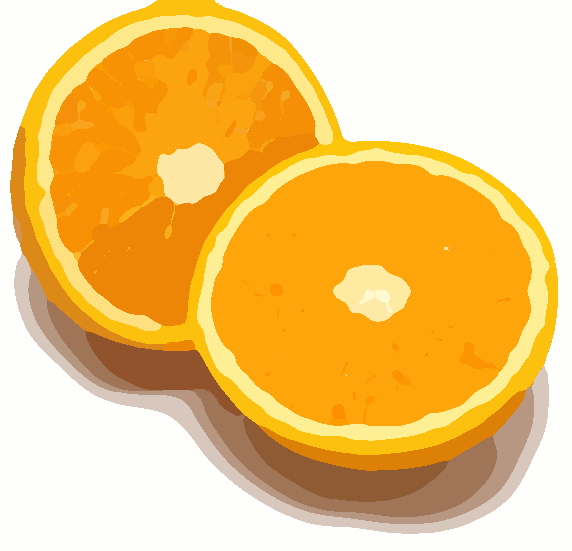
\includegraphics[scale=0.4]{./images/02/orange/meanshift1_5_4.png}
      \caption{Image \texttt{orange} segmented with \texttt{mean-shift}.
        $(\sigma_s^2, \sigma_c^2) \equiv (5.0, 4.0)$}
      \label{fig:02_orange1_5_4}
    \end{figure}
  \end{minipage}
  \hfill
  \begin{minipage}{0.45\linewidth}
    \begin{figure}[H]
      \centering
      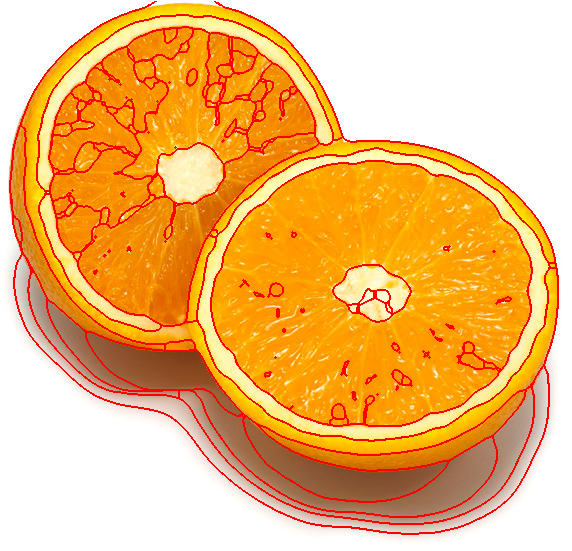
\includegraphics[scale=0.4]{./images/02/orange/meanshift2_5_4.png}
      \caption{Segmentation bounds of image \texttt{orange}.
        $(\sigma_s^2, \sigma_c^2) \equiv (5.0, 4.0)$}
      \label{fig:02_orange2_5_4}
    \end{figure}
  \end{minipage}
\end{minipage}
}

\noindent\makebox[\textwidth][c]{%
\begin{minipage}{\linewidth}
  \begin{minipage}{0.45\linewidth}
    \begin{figure}[H]
      \centering
      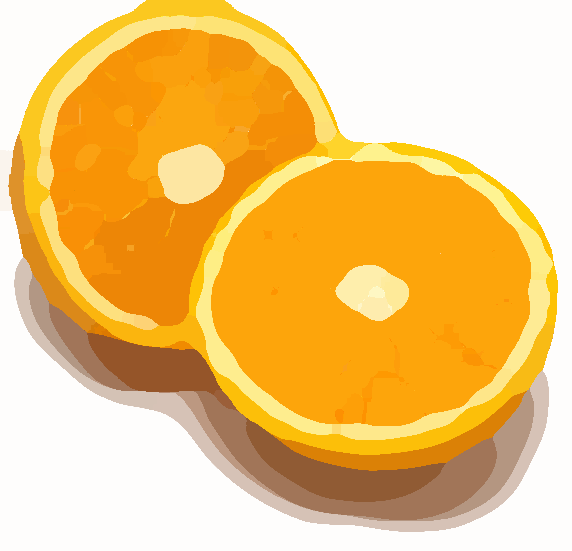
\includegraphics[scale=0.4]{./images/02/orange/meanshift1_8_4.png}
      \caption{Image \texttt{orange} segmented with \texttt{mean-shift}.
        $(\sigma_s^2, \sigma_c^2) \equiv (8.0, 4.0)$}
      \label{fig:02_orange1_8_4}
    \end{figure}
  \end{minipage}
  \hfill
  \begin{minipage}{0.45\linewidth}
    \begin{figure}[H]
      \centering
      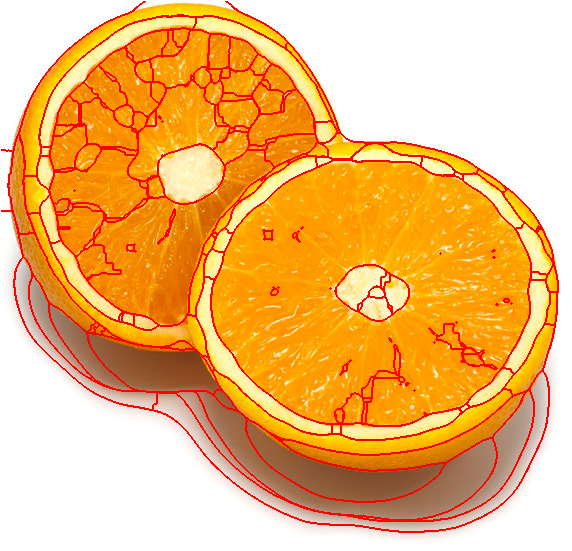
\includegraphics[scale=0.4]{./images/02/orange/meanshift2_8_4.png}
      \caption{Segmentation bounds of image \texttt{orange}.
        $(\sigma_s^2, \sigma_c^2) \equiv (8.0, 4.0)$}
      \label{fig:02_orange2_8_4}
    \end{figure}
  \end{minipage}
\end{minipage}
}

\noindent\makebox[\textwidth][c]{%
\begin{minipage}{\linewidth}
  \begin{minipage}{0.45\linewidth}
    \begin{figure}[H]
      \centering
      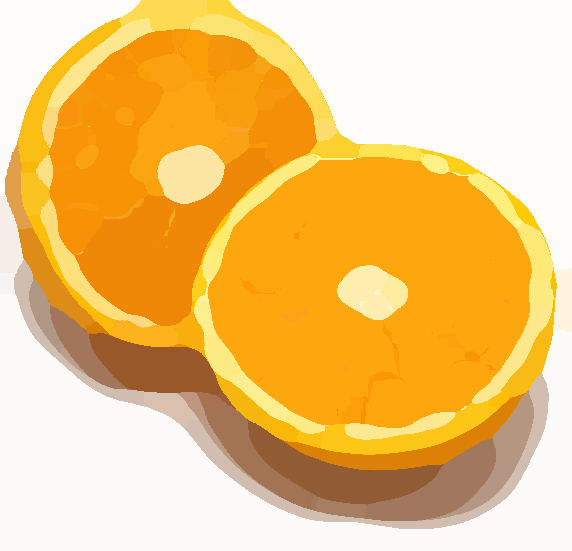
\includegraphics[scale=0.4]{./images/02/orange/meanshift1_10_4.png}
      \caption{Image \texttt{orange} segmented with \texttt{mean-shift}.
        $(\sigma_s^2, \sigma_c^2) \equiv (10.0, 4.0)$}
      \label{fig:02_orange1_10_4}
    \end{figure}
  \end{minipage}
  \hfill
  \begin{minipage}{0.45\linewidth}
    \begin{figure}[H]
      \centering
      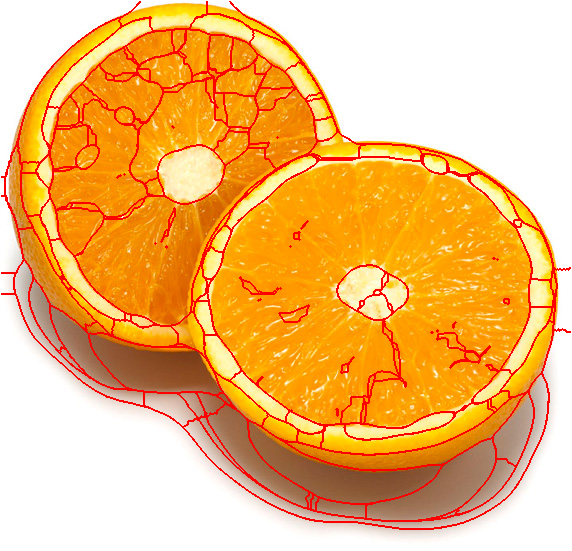
\includegraphics[scale=0.4]{./images/02/orange/meanshift2_10_4.png}
      \caption{Segmentation bounds of image \texttt{orange}.
        $(\sigma_s^2, \sigma_c^2) \equiv (10.0, 4.0)$}
      \label{fig:02_orange2_10_4}
    \end{figure}
  \end{minipage}
\end{minipage}
}

\noindent\makebox[\textwidth][c]{%
\begin{minipage}{\linewidth}
  \begin{minipage}{0.45\linewidth}
    \begin{figure}[H]
      \centering
      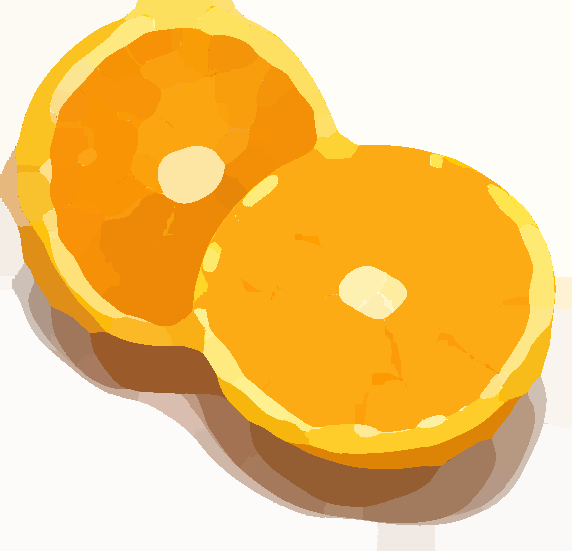
\includegraphics[scale=0.4]{./images/02/orange/meanshift1_12_4.png}
      \caption{Image \texttt{orange} segmented with \texttt{mean-shift}.
        $(\sigma_s^2, \sigma_c^2) \equiv (12.0, 4.0)$}
      \label{fig:02_orange1_12_4}
    \end{figure}
  \end{minipage}
  \hfill
  \begin{minipage}{0.45\linewidth}
    \begin{figure}[H]
      \centering
      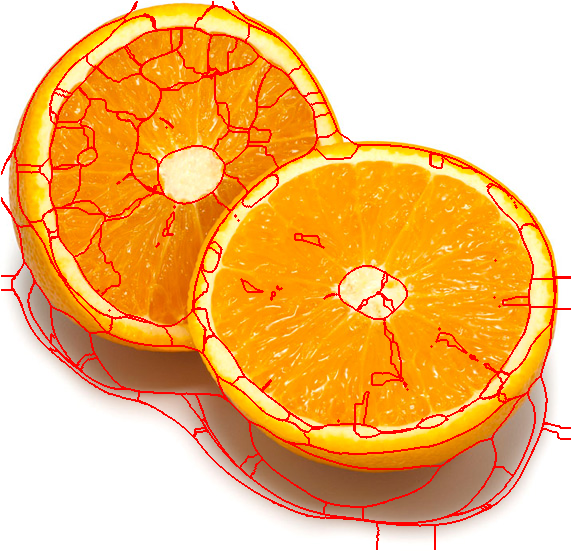
\includegraphics[scale=0.4]{./images/02/orange/meanshift2_12_4.png}
      \caption{Segmentation bounds of image \texttt{orange}.
        $(\sigma_s^2, \sigma_c^2) \equiv (12.0, 4.0)$}
      \label{fig:02_orange2_12_4}
    \end{figure}
  \end{minipage}
\end{minipage}
}

\noindent\makebox[\textwidth][c]{%
\begin{minipage}{\linewidth}
  \begin{minipage}{0.45\linewidth}
    \begin{figure}[H]
      \centering
      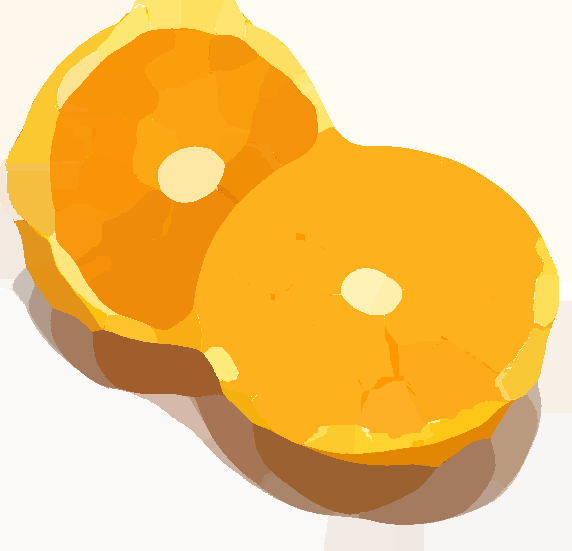
\includegraphics[scale=0.4]{./images/02/orange/meanshift1_15_4.png}
      \caption{Image \texttt{orange} segmented with \texttt{mean-shift}.
        $(\sigma_s^2, \sigma_c^2) \equiv (15.0, 4.0)$}
      \label{fig:02_orange1_15_4}
    \end{figure}
  \end{minipage}
  \hfill
  \begin{minipage}{0.45\linewidth}
    \begin{figure}[H]
      \centering
      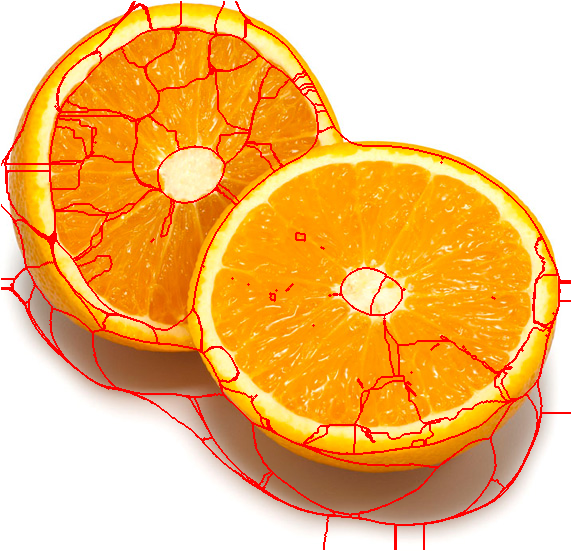
\includegraphics[scale=0.4]{./images/02/orange/meanshift2_15_4.png}
      \caption{Segmentation bounds of image \texttt{orange}.
        $(\sigma_s^2, \sigma_c^2) \equiv (15.0, 4.0)$}
      \label{fig:02_orange2_15_4}
    \end{figure}
  \end{minipage}
\end{minipage}
}

\noindent\makebox[\textwidth][c]{%
\begin{minipage}{\linewidth}
  \begin{minipage}{0.45\linewidth}
    \begin{figure}[H]
      \centering
      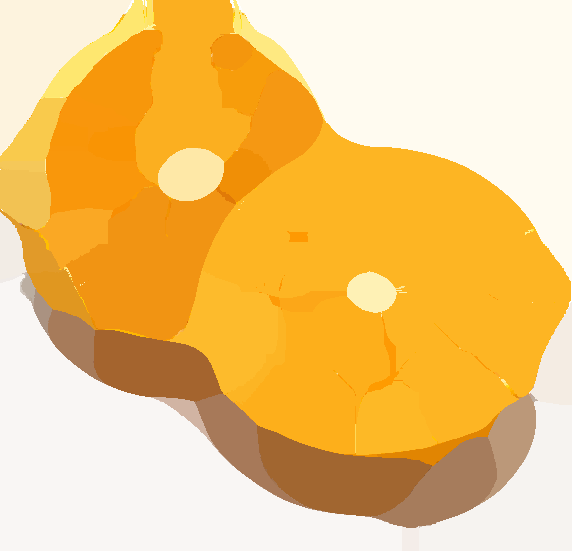
\includegraphics[scale=0.4]{./images/02/orange/meanshift1_20_4.png}
      \caption{Image \texttt{orange} segmented with \texttt{mean-shift}.
        $(\sigma_s^2, \sigma_c^2) \equiv (20.0, 4.0)$}
      \label{fig:02_orange1_20_4}
    \end{figure}
  \end{minipage}
  \hfill
  \begin{minipage}{0.45\linewidth}
    \begin{figure}[H]
      \centering
      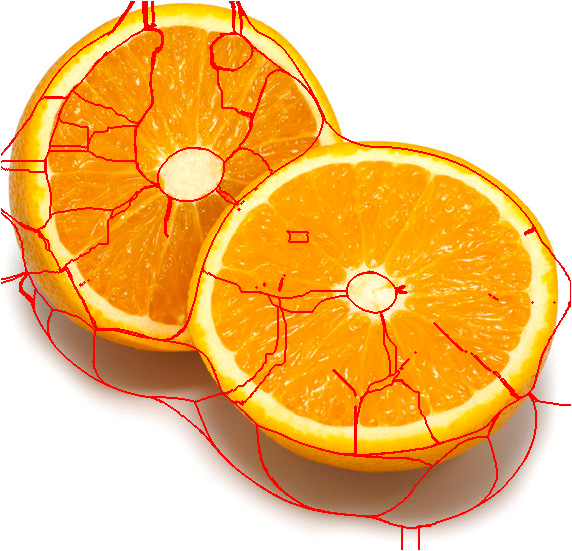
\includegraphics[scale=0.4]{./images/02/orange/meanshift2_20_4.png}
      \caption{Segmentation bounds of image \texttt{orange}.
        $(\sigma_s^2, \sigma_c^2) \equiv (20.0, 4.0)$}
      \label{fig:02_orange2_20_4}
    \end{figure}
  \end{minipage}
\end{minipage}
}


\subsubsection{Image \texttt{orange}. Varying $\sigma_c^2$.}

\noindent\makebox[\textwidth][c]{%
\begin{minipage}{\linewidth}
  \begin{minipage}{0.45\linewidth}
    \begin{figure}[H]
      \centering
      
\includegraphics[scale=0.4]{./images/02/orange/meanshift1_8_1.png}
      \caption{Image \texttt{orange} segmented with \texttt{mean-shift}.
        $(\sigma_s^2, \sigma_c^2) \equiv (8.0, 1.0)$}
      \label{fig:02_orange1_8_1}
    \end{figure}
  \end{minipage}
  \hfill
  \begin{minipage}{0.45\linewidth}
    \begin{figure}[H]
      \centering
      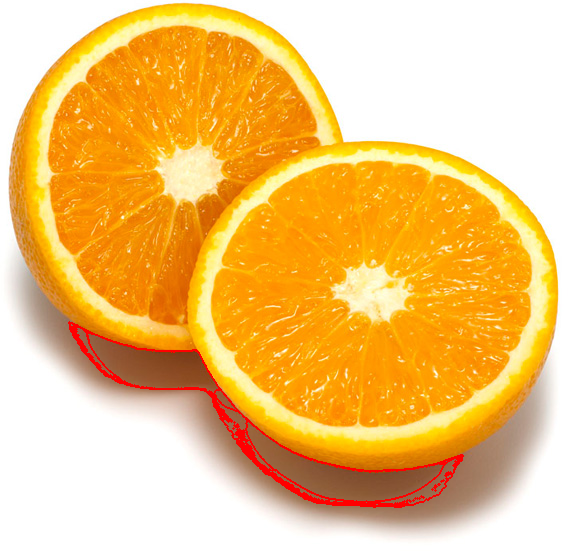
\includegraphics[scale=0.4]{./images/02/orange/meanshift2_8_1.png}
      \caption{Segmentation bounds of image \texttt{orange}.
        $(\sigma_s^2, \sigma_c^2) \equiv (8.0, 1.0)$}
      \label{fig:02_orange2_8_1}
    \end{figure}
  \end{minipage}
\end{minipage}
}

\noindent\makebox[\textwidth][c]{%
\begin{minipage}{\linewidth}
  \begin{minipage}{0.45\linewidth}
    \begin{figure}[H]
      \centering
      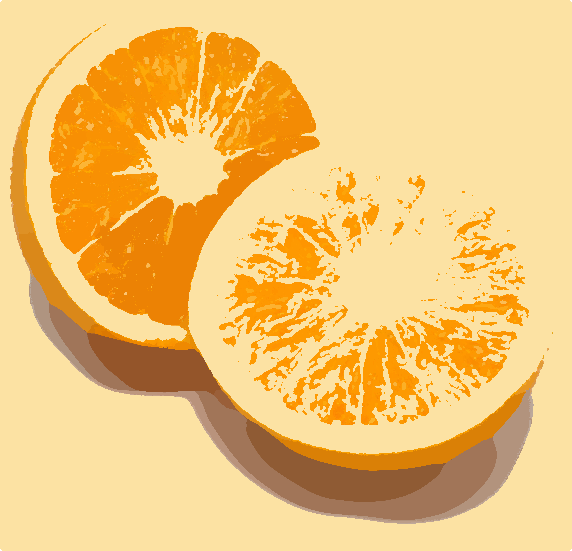
\includegraphics[scale=0.4]{./images/02/orange/meanshift1_8_1.2.png}
      \caption{Image \texttt{orange} segmented with \texttt{mean-shift}.
        $(\sigma_s^2, \sigma_c^2) \equiv (8.0, 1.2)$}
      \label{fig:02_orange1_8_1.2}
    \end{figure}
  \end{minipage}
  \hfill
  \begin{minipage}{0.45\linewidth}
    \begin{figure}[H]
      \centering
      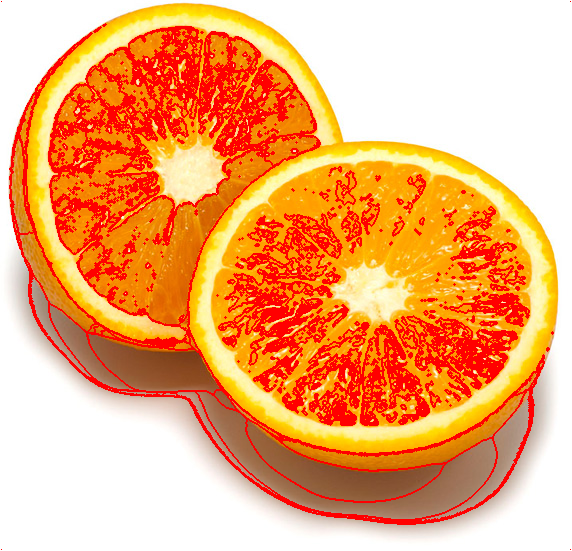
\includegraphics[scale=0.4]{./images/02/orange/meanshift2_8_1.2.png}
      \caption{Segmentation bounds of image \texttt{orange}.
        $(\sigma_s^2, \sigma_c^2) \equiv (8.0, 1.2)$}
      \label{fig:02_orange2_8_1.2}
    \end{figure}
  \end{minipage}
\end{minipage}
}

\noindent\makebox[\textwidth][c]{%
\begin{minipage}{\linewidth}
  \begin{minipage}{0.45\linewidth}
    \begin{figure}[H]
      \centering
      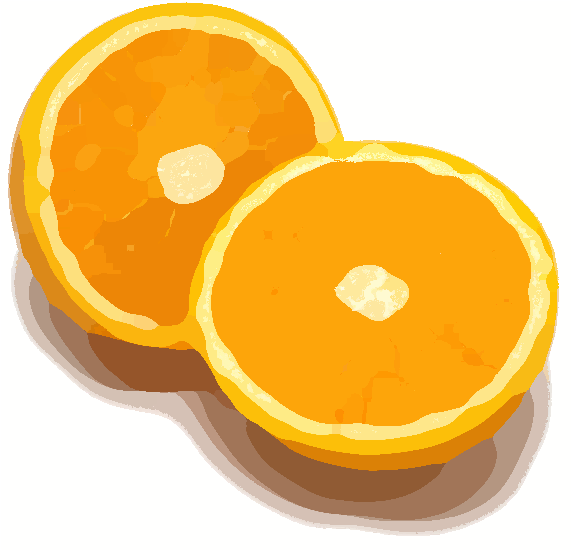
\includegraphics[scale=0.4]{./images/02/orange/meanshift1_8_1.4.png}
      \caption{Image \texttt{orange} segmented with \texttt{mean-shift}.
        $(\sigma_s^2, \sigma_c^2) \equiv (8.0, 1.4)$}
      \label{fig:02_orange1_8_1.4}
    \end{figure}
  \end{minipage}
  \hfill
  \begin{minipage}{0.45\linewidth}
    \begin{figure}[H]
      \centering
      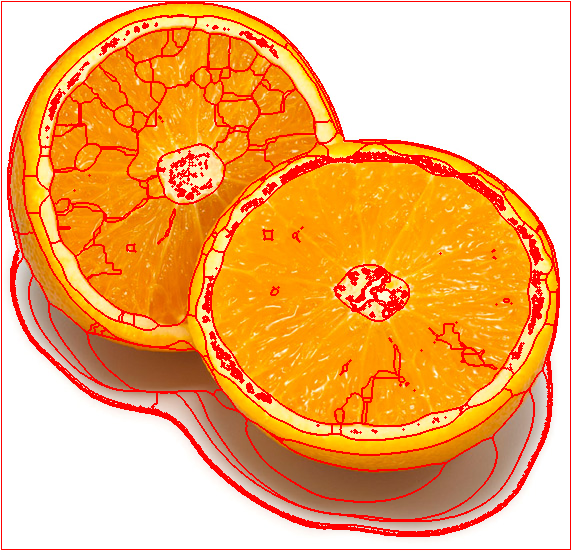
\includegraphics[scale=0.4]{./images/02/orange/meanshift2_8_1.4.png}
      \caption{Segmentation bounds of image \texttt{orange}.
        $(\sigma_s^2, \sigma_c^2) \equiv (8.0, 1.4)$}
      \label{fig:02_orange2_8_1.4}
    \end{figure}
  \end{minipage}
\end{minipage}
}

\noindent\makebox[\textwidth][c]{%
\begin{minipage}{\linewidth}
  \begin{minipage}{0.45\linewidth}
    \begin{figure}[H]
      \centering
      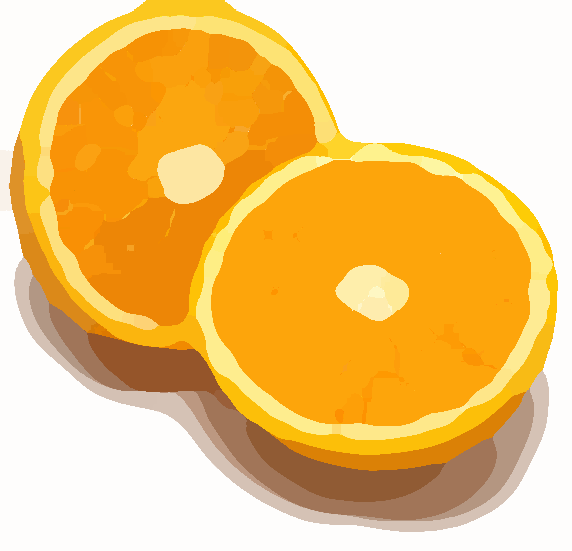
\includegraphics[scale=0.4]{./images/02/orange/meanshift1_8_1.6.png}
      \caption{Image \texttt{orange} segmented with \texttt{mean-shift}.
        $(\sigma_s^2, \sigma_c^2) \equiv (8.0, 1.6)$}
      \label{fig:02_orange1_8_1.6}
    \end{figure}
  \end{minipage}
  \hfill
  \begin{minipage}{0.45\linewidth}
    \begin{figure}[H]
      \centering
      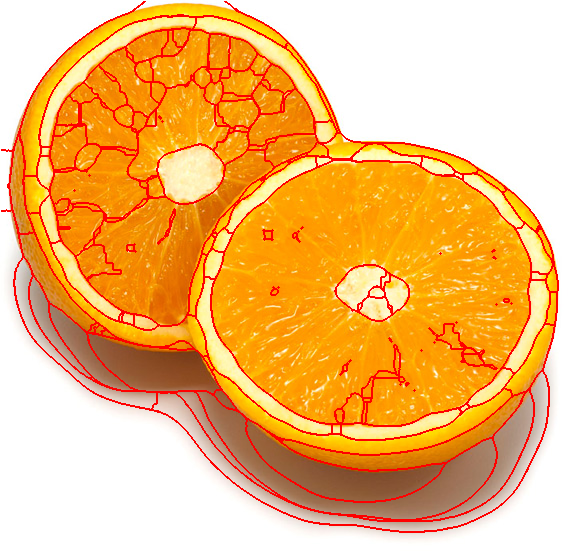
\includegraphics[scale=0.4]{./images/02/orange/meanshift2_8_1.6.png}
      \caption{Segmentation bounds of image \texttt{orange}.
        $(\sigma_s^2, \sigma_c^2) \equiv (8.0, 1.6)$}
      \label{fig:02_orange2_8_1.6}
    \end{figure}
  \end{minipage}
\end{minipage}
}

\noindent\makebox[\textwidth][c]{%
\begin{minipage}{\linewidth}
  \begin{minipage}{0.45\linewidth}
    \begin{figure}[H]
      \centering
      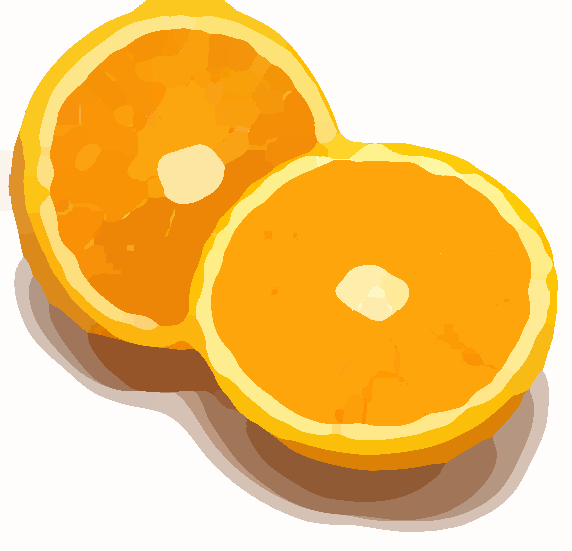
\includegraphics[scale=0.4]{./images/02/orange/meanshift1_8_1.8.png}
      \caption{Image \texttt{orange} segmented with \texttt{mean-shift}.
        $(\sigma_s^2, \sigma_c^2) \equiv (8.0, 1.8)$}
      \label{fig:02_orange1_8_1.8}
    \end{figure}
  \end{minipage}
  \hfill
  \begin{minipage}{0.45\linewidth}
    \begin{figure}[H]
      \centering
      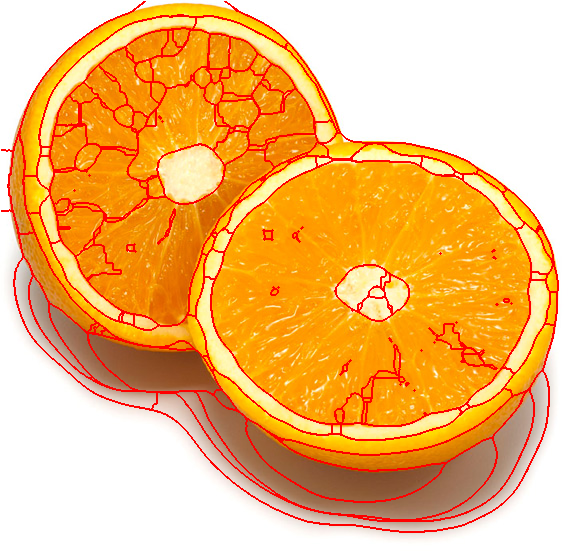
\includegraphics[scale=0.4]{./images/02/orange/meanshift2_8_1.8.png}
      \caption{Segmentation bounds of image \texttt{orange}.
        $(\sigma_s^2, \sigma_c^2) \equiv (8.0, 1.8)$}
      \label{fig:02_orange2_8_1.8}
    \end{figure}
  \end{minipage}
\end{minipage}
}

\noindent\makebox[\textwidth][c]{%
\begin{minipage}{\linewidth}
  \begin{minipage}{0.45\linewidth}
    \begin{figure}[H]
      \centering
      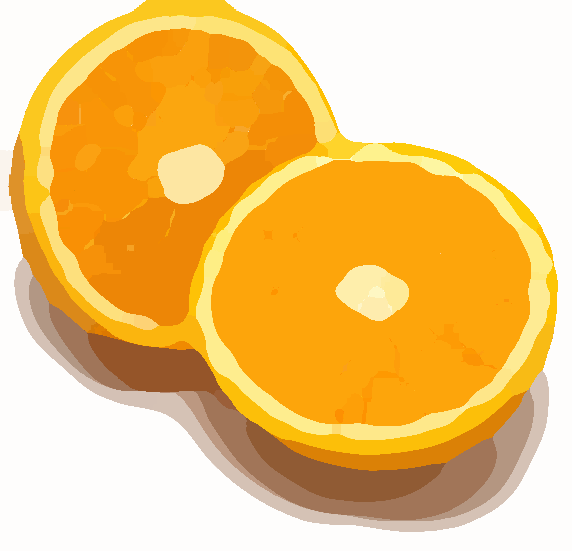
\includegraphics[scale=0.4]{./images/02/orange/meanshift1_8_2.png}
      \caption{Image \texttt{orange} segmented with \texttt{mean-shift}.
        $(\sigma_s^2, \sigma_c^2) \equiv (8.0, 2.0)$}
      \label{fig:02_orange1_8_2}
    \end{figure}
  \end{minipage}
  \hfill
  \begin{minipage}{0.45\linewidth}
    \begin{figure}[H]
      \centering
      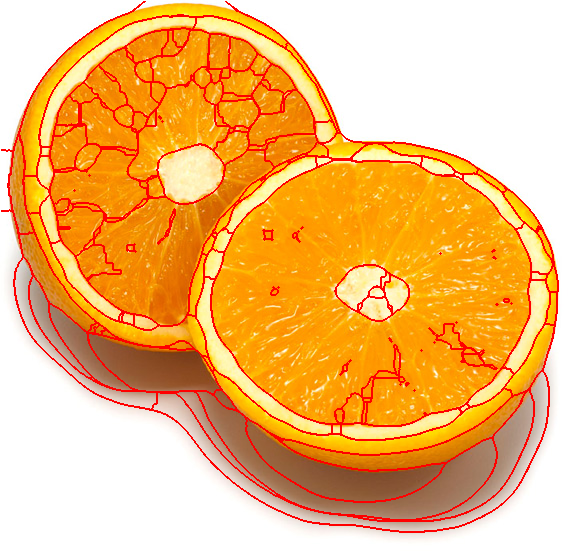
\includegraphics[scale=0.4]{./images/02/orange/meanshift2_8_2.png}
      \caption{Segmentation bounds of image \texttt{orange}.
        $(\sigma_s^2, \sigma_c^2) \equiv (8.0, 2.0)$}
      \label{fig:02_orange2_8_2}
    \end{figure}
  \end{minipage}
\end{minipage}
}


% ----------------------------------- tiger1 -----------------------------------
\subsubsection{Image \texttt{tiger1}. Varying $\sigma_s^2$.}

\noindent\makebox[\textwidth][c]{%
\begin{minipage}{\linewidth}
  \begin{minipage}{0.45\linewidth}
    \begin{figure}[H]
      \centering
      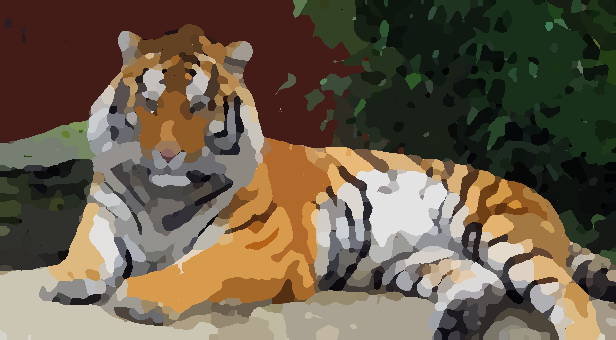
\includegraphics[scale=0.35]{./images/02/tiger1/meanshift1_3_4.png}
      \caption{Image \texttt{tiger1} segmented with \texttt{mean-shift}.
        $(\sigma_s^2, \sigma_c^2) \equiv (3.0, 4.0)$}
      \label{fig:02_tiger1_1_3_4}
    \end{figure}
  \end{minipage}
  \hfill
  \begin{minipage}{0.45\linewidth}
    \begin{figure}[H]
      \centering
      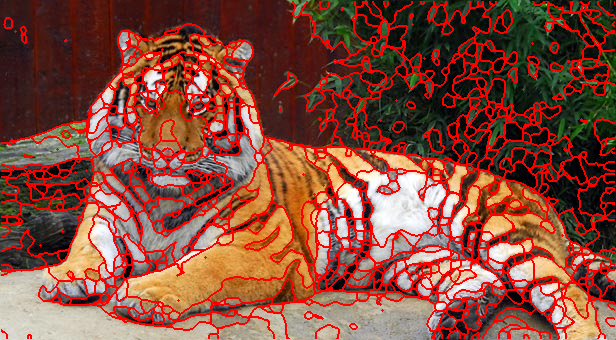
\includegraphics[scale=0.35]{./images/02/tiger1/meanshift2_3_4.png}
      \caption{Segmentation bounds of image \texttt{tiger1}.
        $(\sigma_s^2, \sigma_c^2) \equiv (3.0, 4.0)$}
      \label{fig:02_tiger1_2_3_4}
    \end{figure}
  \end{minipage}
\end{minipage}
}

\noindent\makebox[\textwidth][c]{%
\begin{minipage}{\linewidth}
  \begin{minipage}{0.45\linewidth}
    \begin{figure}[H]
      \centering
      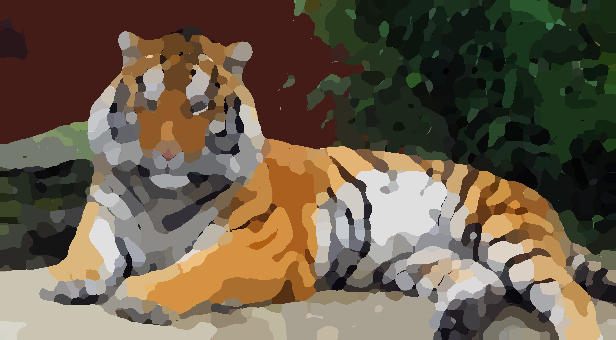
\includegraphics[scale=0.35]{./images/02/tiger1/meanshift1_4_4.png}
      \caption{Image \texttt{tiger1} segmented with \texttt{mean-shift}.
        $(\sigma_s^2, \sigma_c^2) \equiv (4.0, 4.0)$}
      \label{fig:02_tiger1_1_4_4}
    \end{figure}
  \end{minipage}
  \hfill
  \begin{minipage}{0.45\linewidth}
    \begin{figure}[H]
      \centering
      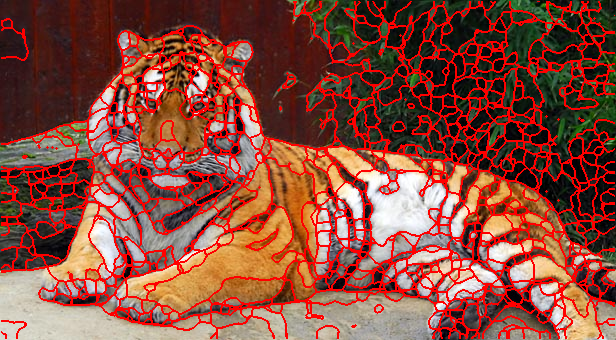
\includegraphics[scale=0.35]{./images/02/tiger1/meanshift2_4_4.png}
      \caption{Segmentation bounds of image \texttt{tiger1}.
        $(\sigma_s^2, \sigma_c^2) \equiv (4.0, 4.0)$}
      \label{fig:02_tiger1_2_4_4}
    \end{figure}
  \end{minipage}
\end{minipage}
}

\noindent\makebox[\textwidth][c]{%
\begin{minipage}{\linewidth}
  \begin{minipage}{0.45\linewidth}
    \begin{figure}[H]
      \centering
      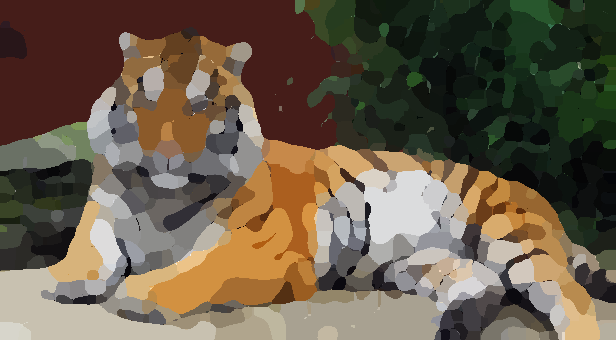
\includegraphics[scale=0.35]{./images/02/tiger1/meanshift1_5_4.png}
      \caption{Image \texttt{tiger1} segmented with \texttt{mean-shift}.
        $(\sigma_s^2, \sigma_c^2) \equiv (5.0, 4.0)$}
      \label{fig:02_tiger1_1_5_4}
    \end{figure}
  \end{minipage}
  \hfill
  \begin{minipage}{0.45\linewidth}
    \begin{figure}[H]
      \centering
      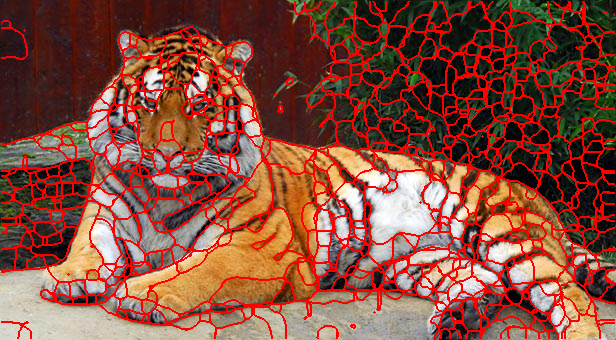
\includegraphics[scale=0.35]{./images/02/tiger1/meanshift2_5_4.png}
      \caption{Segmentation bounds of image \texttt{tiger1}.
        $(\sigma_s^2, \sigma_c^2) \equiv (5.0, 4.0)$}
      \label{fig:02_tiger1_2_5_4}
    \end{figure}
  \end{minipage}
\end{minipage}
}

\noindent\makebox[\textwidth][c]{%
\begin{minipage}{\linewidth}
  \begin{minipage}{0.45\linewidth}
    \begin{figure}[H]
      \centering
      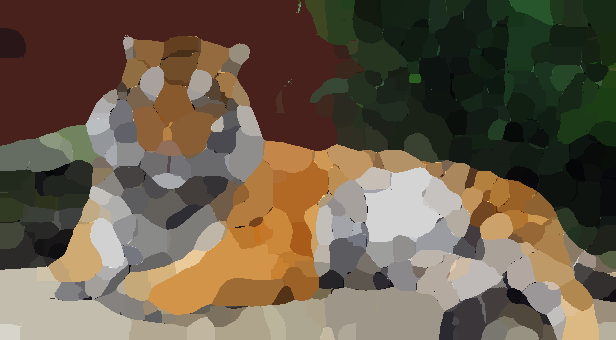
\includegraphics[scale=0.35]{./images/02/tiger1/meanshift1_8_4.png}
      \caption{Image \texttt{tiger1} segmented with \texttt{mean-shift}.
        $(\sigma_s^2, \sigma_c^2) \equiv (8.0, 4.0)$}
      \label{fig:02_tiger1_1_8_4}
    \end{figure}
  \end{minipage}
  \hfill
  \begin{minipage}{0.45\linewidth}
    \begin{figure}[H]
      \centering
      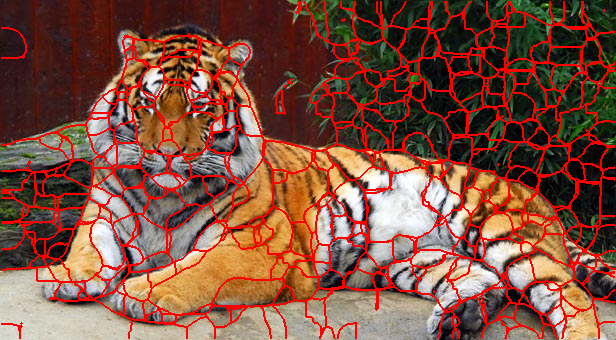
\includegraphics[scale=0.35]{./images/02/tiger1/meanshift2_8_4.png}
      \caption{Segmentation bounds of image \texttt{tiger1}.
        $(\sigma_s^2, \sigma_c^2) \equiv (8.0, 4.0)$}
      \label{fig:02_tiger1_2_8_4}
    \end{figure}
  \end{minipage}
\end{minipage}
}

\noindent\makebox[\textwidth][c]{%
\begin{minipage}{\linewidth}
  \begin{minipage}{0.45\linewidth}
    \begin{figure}[H]
      \centering
      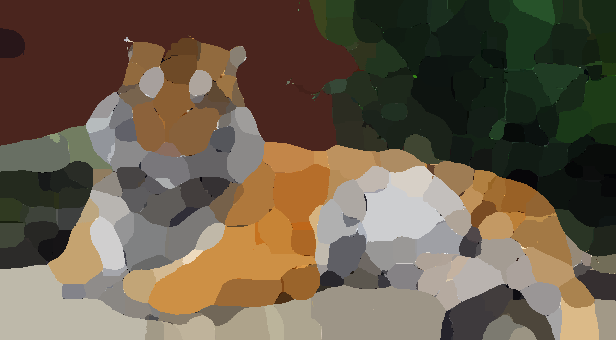
\includegraphics[scale=0.35]{./images/02/tiger1/meanshift1_10_4.png}
      \caption{Image \texttt{tiger1} segmented with \texttt{mean-shift}.
        $(\sigma_s^2, \sigma_c^2) \equiv (10.0, 4.0)$}
      \label{fig:02_tiger1_1_10_4}
    \end{figure}
  \end{minipage}
  \hfill
  \begin{minipage}{0.45\linewidth}
    \begin{figure}[H]
      \centering
      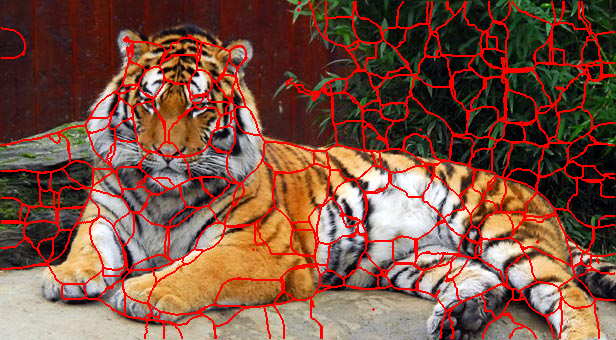
\includegraphics[scale=0.35]{./images/02/tiger1/meanshift2_10_4.png}
      \caption{Segmentation bounds of image \texttt{tiger1}.
        $(\sigma_s^2, \sigma_c^2) \equiv (10.0, 4.0)$}
      \label{fig:02_tiger1_2_10_4}
    \end{figure}
  \end{minipage}
\end{minipage}
}

\noindent\makebox[\textwidth][c]{%
\begin{minipage}{\linewidth}
  \begin{minipage}{0.45\linewidth}
    \begin{figure}[H]
      \centering
      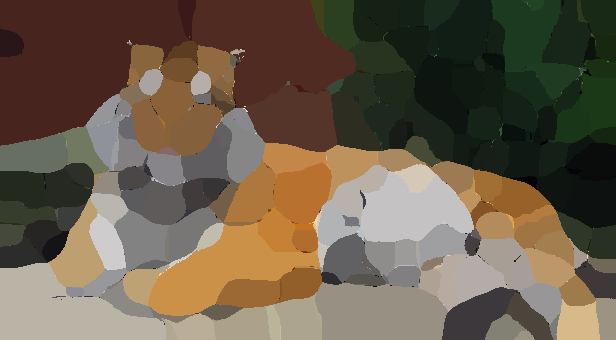
\includegraphics[scale=0.35]{./images/02/tiger1/meanshift1_12_4.png}
      \caption{Image \texttt{tiger1} segmented with \texttt{mean-shift}.
        $(\sigma_s^2, \sigma_c^2) \equiv (12.0, 4.0)$}
      \label{fig:02_tiger1_1_12_4}
    \end{figure}
  \end{minipage}
  \hfill
  \begin{minipage}{0.45\linewidth}
    \begin{figure}[H]
      \centering
      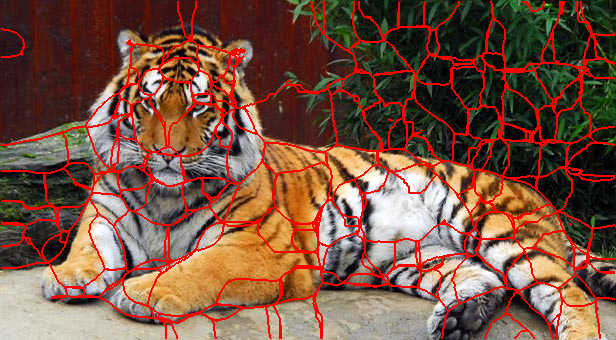
\includegraphics[scale=0.35]{./images/02/tiger1/meanshift2_12_4.png}
      \caption{Segmentation bounds of image \texttt{tiger1}.
        $(\sigma_s^2, \sigma_c^2) \equiv (12.0, 4.0)$}
      \label{fig:02_tiger1_2_12_4}
    \end{figure}
  \end{minipage}
\end{minipage}
}

\noindent\makebox[\textwidth][c]{%
\begin{minipage}{\linewidth}
  \begin{minipage}{0.45\linewidth}
    \begin{figure}[H]
      \centering
      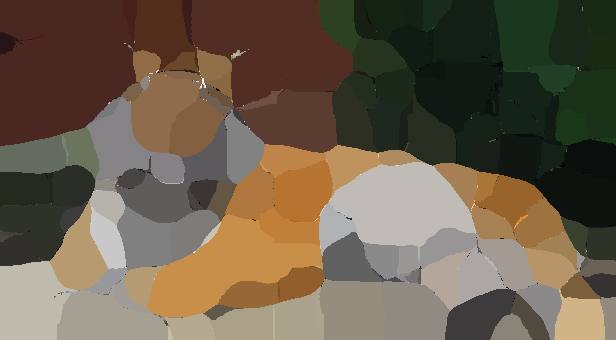
\includegraphics[scale=0.35]{./images/02/tiger1/meanshift1_15_4.png}
      \caption{Image \texttt{tiger1} segmented with \texttt{mean-shift}.
        $(\sigma_s^2, \sigma_c^2) \equiv (15.0, 4.0)$}
      \label{fig:02_tiger1_1_15_4}
    \end{figure}
  \end{minipage}
  \hfill
  \begin{minipage}{0.45\linewidth}
    \begin{figure}[H]
      \centering
      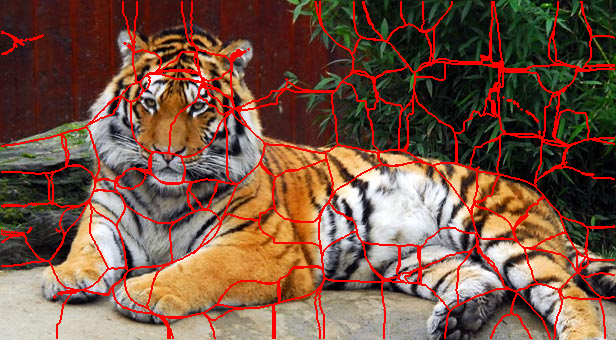
\includegraphics[scale=0.35]{./images/02/tiger1/meanshift2_15_4.png}
      \caption{Segmentation bounds of image \texttt{tiger1}.
        $(\sigma_s^2, \sigma_c^2) \equiv (15.0, 4.0)$}
      \label{fig:02_tiger1_2_15_4}
    \end{figure}
  \end{minipage}
\end{minipage}
}

\noindent\makebox[\textwidth][c]{%
\begin{minipage}{\linewidth}
  \begin{minipage}{0.45\linewidth}
    \begin{figure}[H]
      \centering
      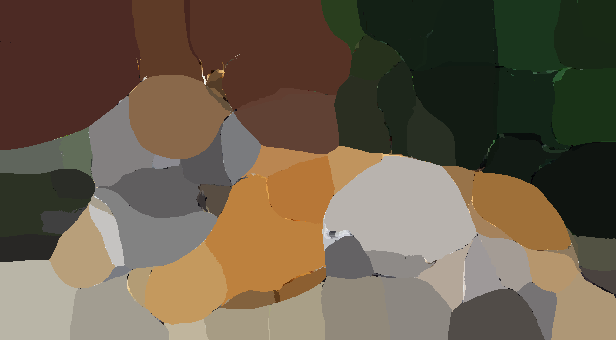
\includegraphics[scale=0.35]{./images/02/tiger1/meanshift1_20_4.png}
      \caption{Image \texttt{tiger1} segmented with \texttt{mean-shift}.
        $(\sigma_s^2, \sigma_c^2) \equiv (20.0, 4.0)$}
      \label{fig:02_tiger1_1_20_4}
    \end{figure}
  \end{minipage}
  \hfill
  \begin{minipage}{0.45\linewidth}
    \begin{figure}[H]
      \centering
      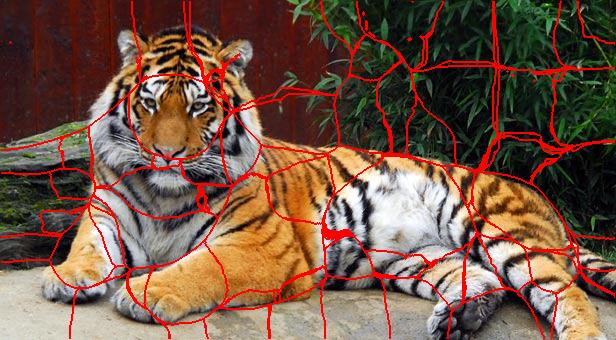
\includegraphics[scale=0.35]{./images/02/tiger1/meanshift2_20_4.png}
      \caption{Segmentation bounds of image \texttt{tiger1}.
        $(\sigma_s^2, \sigma_c^2) \equiv (20.0, 4.0)$}
      \label{fig:02_tiger1_2_20_4}
    \end{figure}
  \end{minipage}
\end{minipage}
}


\subsubsection{Image \texttt{tiger1}. Varying $\sigma_c^2$.}

\noindent\makebox[\textwidth][c]{%
\begin{minipage}{\linewidth}
  \begin{minipage}{0.45\linewidth}
    \begin{figure}[H]
      \centering
      
\includegraphics[scale=0.4]{./images/02/tiger1/meanshift1_8_1.png}
      \caption{Image \texttt{tiger1} segmented with \texttt{mean-shift}.
        $(\sigma_s^2, \sigma_c^2) \equiv (8.0, 1.0)$}
      \label{fig:02_tiger1_1_8_1}
    \end{figure}
  \end{minipage}
  \hfill
  \begin{minipage}{0.45\linewidth}
    \begin{figure}[H]
      \centering
      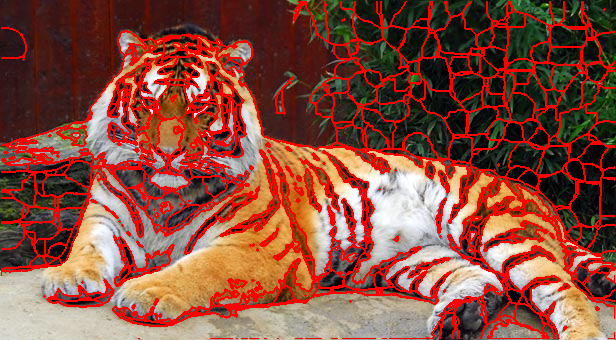
\includegraphics[scale=0.4]{./images/02/tiger1/meanshift2_8_1.png}
      \caption{Segmentation bounds of image \texttt{tiger1}.
        $(\sigma_s^2, \sigma_c^2) \equiv (8.0, 1.0)$}
      \label{fig:02_tiger1_2_8_1}
    \end{figure}
  \end{minipage}
\end{minipage}
}

\noindent\makebox[\textwidth][c]{%
\begin{minipage}{\linewidth}
  \begin{minipage}{0.45\linewidth}
    \begin{figure}[H]
      \centering
      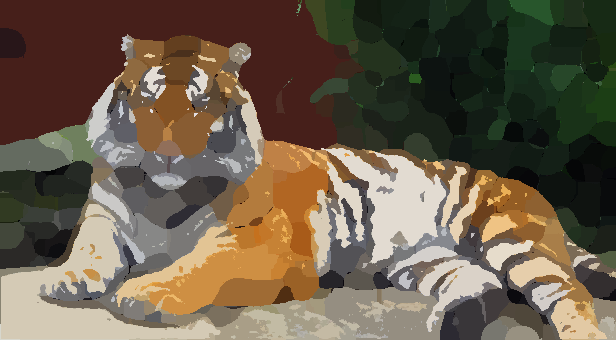
\includegraphics[scale=0.4]{./images/02/tiger1/meanshift1_8_1.2.png}
      \caption{Image \texttt{tiger1} segmented with \texttt{mean-shift}.
        $(\sigma_s^2, \sigma_c^2) \equiv (8.0, 1.2)$}
      \label{fig:02_tiger1_1_8_1.2}
    \end{figure}
  \end{minipage}
  \hfill
  \begin{minipage}{0.45\linewidth}
    \begin{figure}[H]
      \centering
      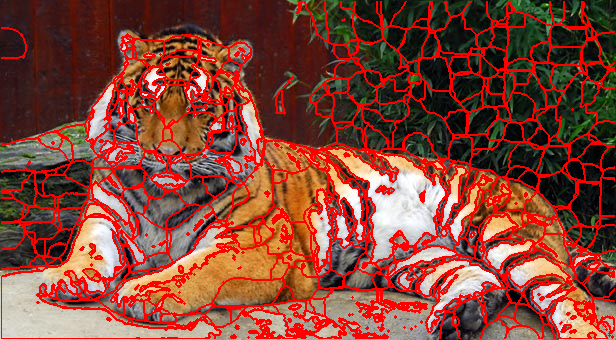
\includegraphics[scale=0.4]{./images/02/tiger1/meanshift2_8_1.2.png}
      \caption{Segmentation bounds of image \texttt{tiger1}.
        $(\sigma_s^2, \sigma_c^2) \equiv (8.0, 1.2)$}
      \label{fig:02_tiger1_2_8_1.2}
    \end{figure}
  \end{minipage}
\end{minipage}
}

\noindent\makebox[\textwidth][c]{%
\begin{minipage}{\linewidth}
  \begin{minipage}{0.45\linewidth}
    \begin{figure}[H]
      \centering
      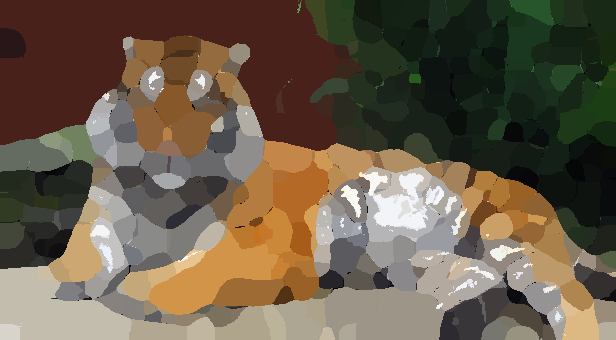
\includegraphics[scale=0.4]{./images/02/tiger1/meanshift1_8_1.4.png}
      \caption{Image \texttt{tiger1} segmented with \texttt{mean-shift}.
        $(\sigma_s^2, \sigma_c^2) \equiv (8.0, 1.4)$}
      \label{fig:02_tiger1_1_8_1.4}
    \end{figure}
  \end{minipage}
  \hfill
  \begin{minipage}{0.45\linewidth}
    \begin{figure}[H]
      \centering
      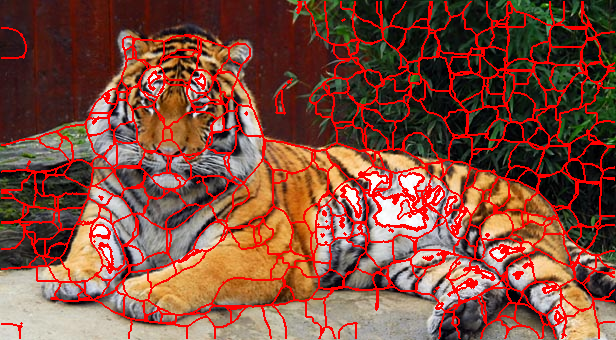
\includegraphics[scale=0.4]{./images/02/tiger1/meanshift2_8_1.4.png}
      \caption{Segmentation bounds of image \texttt{tiger1}.
        $(\sigma_s^2, \sigma_c^2) \equiv (8.0, 1.4)$}
      \label{fig:02_tiger1_2_8_1.4}
    \end{figure}
  \end{minipage}
\end{minipage}
}

\noindent\makebox[\textwidth][c]{%
\begin{minipage}{\linewidth}
  \begin{minipage}{0.45\linewidth}
    \begin{figure}[H]
      \centering
      \includegraphics[scale=0.4]{./images/02/tiger1/meanshift1_8_1.6.png}
      \caption{Image \texttt{tiger1} segmented with \texttt{mean-shift}.
        $(\sigma_s^2, \sigma_c^2) \equiv (8.0, 1.6)$}
      \label{fig:02_tiger1_1_8_1.6}
    \end{figure}
  \end{minipage}
  \hfill
  \begin{minipage}{0.45\linewidth}
    \begin{figure}[H]
      \centering
      \includegraphics[scale=0.4]{./images/02/tiger1/meanshift2_8_1.6.png}
      \caption{Segmentation bounds of image \texttt{tiger1}.
        $(\sigma_s^2, \sigma_c^2) \equiv (8.0, 1.6)$}
      \label{fig:02_tiger1_2_8_1.6}
    \end{figure}
  \end{minipage}
\end{minipage}
}

\noindent\makebox[\textwidth][c]{%
\begin{minipage}{\linewidth}
  \begin{minipage}{0.45\linewidth}
    \begin{figure}[H]
      \centering
      \includegraphics[scale=0.4]{./images/02/tiger1/meanshift1_8_1.8.png}
      \caption{Image \texttt{tiger1} segmented with \texttt{mean-shift}.
        $(\sigma_s^2, \sigma_c^2) \equiv (8.0, 1.8)$}
      \label{fig:02_tiger1_1_8_1.8}
    \end{figure}
  \end{minipage}
  \hfill
  \begin{minipage}{0.45\linewidth}
    \begin{figure}[H]
      \centering
      \includegraphics[scale=0.4]{./images/02/tiger1/meanshift2_8_1.8.png}
      \caption{Segmentation bounds of image \texttt{tiger1}.
        $(\sigma_s^2, \sigma_c^2) \equiv (8.0, 1.8)$}
      \label{fig:02_tiger1_2_8_1.8}
    \end{figure}
  \end{minipage}
\end{minipage}
}

\noindent\makebox[\textwidth][c]{%
\begin{minipage}{\linewidth}
  \begin{minipage}{0.45\linewidth}
    \begin{figure}[H]
      \centering
      \includegraphics[scale=0.4]{./images/02/tiger1/meanshift1_8_2.png}
      \caption{Image \texttt{tiger1} segmented with \texttt{mean-shift}.
        $(\sigma_s^2, \sigma_c^2) \equiv (8.0, 2.0)$}
      \label{fig:02_tiger1_1_8_2}
    \end{figure}
  \end{minipage}
  \hfill
  \begin{minipage}{0.45\linewidth}
    \begin{figure}[H]
      \centering
      \includegraphics[scale=0.4]{./images/02/tiger1/meanshift2_8_2.png}
      \caption{Segmentation bounds of image \texttt{tiger1}.
        $(\sigma_s^2, \sigma_c^2) \equiv (8.0, 2.0)$}
      \label{fig:02_tiger1_2_8_2}
    \end{figure}
  \end{minipage}
\end{minipage}
}

% ----------------------------------- tiger2 -----------------------------------
\subsubsection{Image \texttt{tiger2}. Varying $\sigma_s^2$.}

\noindent\makebox[\textwidth][c]{%
\begin{minipage}{\linewidth}
  \begin{minipage}{0.45\linewidth}
    \begin{figure}[H]
      \centering
      \includegraphics[scale=0.35]{./images/02/tiger2/meanshift1_3_4.png}
      \caption{Image \texttt{tiger2} segmented with \texttt{mean-shift}.
        $(\sigma_s^2, \sigma_c^2) \equiv (3.0, 4.0)$}
      \label{fig:02_tiger2_1_3_4}
    \end{figure}
  \end{minipage}
  \hfill
  \begin{minipage}{0.45\linewidth}
    \begin{figure}[H]
      \centering
      \includegraphics[scale=0.35]{./images/02/tiger2/meanshift2_3_4.png}
      \caption{Segmentation bounds of image \texttt{tiger2}.
        $(\sigma_s^2, \sigma_c^2) \equiv (3.0, 4.0)$}
      \label{fig:02_tiger2_2_3_4}
    \end{figure}
  \end{minipage}
\end{minipage}
}

\noindent\makebox[\textwidth][c]{%
\begin{minipage}{\linewidth}
  \begin{minipage}{0.45\linewidth}
    \begin{figure}[H]
      \centering
      \includegraphics[scale=0.35]{./images/02/tiger2/meanshift1_4_4.png}
      \caption{Image \texttt{tiger2} segmented with \texttt{mean-shift}.
        $(\sigma_s^2, \sigma_c^2) \equiv (4.0, 4.0)$}
      \label{fig:02_tiger2_1_4_4}
    \end{figure}
  \end{minipage}
  \hfill
  \begin{minipage}{0.45\linewidth}
    \begin{figure}[H]
      \centering
      \includegraphics[scale=0.35]{./images/02/tiger2/meanshift2_4_4.png}
      \caption{Segmentation bounds of image \texttt{tiger2}.
        $(\sigma_s^2, \sigma_c^2) \equiv (4.0, 4.0)$}
      \label{fig:02_tiger2_2_4_4}
    \end{figure}
  \end{minipage}
\end{minipage}
}

\noindent\makebox[\textwidth][c]{%
\begin{minipage}{\linewidth}
  \begin{minipage}{0.45\linewidth}
    \begin{figure}[H]
      \centering
      \includegraphics[scale=0.35]{./images/02/tiger2/meanshift1_5_4.png}
      \caption{Image \texttt{tiger2} segmented with \texttt{mean-shift}.
        $(\sigma_s^2, \sigma_c^2) \equiv (5.0, 4.0)$}
      \label{fig:02_tiger2_1_5_4}
    \end{figure}
  \end{minipage}
  \hfill
  \begin{minipage}{0.45\linewidth}
    \begin{figure}[H]
      \centering
      \includegraphics[scale=0.35]{./images/02/tiger2/meanshift2_5_4.png}
      \caption{Segmentation bounds of image \texttt{tiger2}.
        $(\sigma_s^2, \sigma_c^2) \equiv (5.0, 4.0)$}
      \label{fig:02_tiger2_2_5_4}
    \end{figure}
  \end{minipage}
\end{minipage}
}

\noindent\makebox[\textwidth][c]{%
\begin{minipage}{\linewidth}
  \begin{minipage}{0.45\linewidth}
    \begin{figure}[H]
      \centering
      \includegraphics[scale=0.35]{./images/02/tiger2/meanshift1_8_4.png}
      \caption{Image \texttt{tiger2} segmented with \texttt{mean-shift}.
        $(\sigma_s^2, \sigma_c^2) \equiv (8.0, 4.0)$}
      \label{fig:02_tiger2_1_8_4}
    \end{figure}
  \end{minipage}
  \hfill
  \begin{minipage}{0.45\linewidth}
    \begin{figure}[H]
      \centering
      \includegraphics[scale=0.35]{./images/02/tiger2/meanshift2_8_4.png}
      \caption{Segmentation bounds of image \texttt{tiger2}.
        $(\sigma_s^2, \sigma_c^2) \equiv (8.0, 4.0)$}
      \label{fig:02_tiger2_2_8_4}
    \end{figure}
  \end{minipage}
\end{minipage}
}

\noindent\makebox[\textwidth][c]{%
\begin{minipage}{\linewidth}
  \begin{minipage}{0.45\linewidth}
    \begin{figure}[H]
      \centering
      \includegraphics[scale=0.35]{./images/02/tiger2/meanshift1_10_4.png}
      \caption{Image \texttt{tiger2} segmented with \texttt{mean-shift}.
        $(\sigma_s^2, \sigma_c^2) \equiv (10.0, 4.0)$}
      \label{fig:02_tiger2_1_10_4}
    \end{figure}
  \end{minipage}
  \hfill
  \begin{minipage}{0.45\linewidth}
    \begin{figure}[H]
      \centering
      \includegraphics[scale=0.35]{./images/02/tiger2/meanshift2_10_4.png}
      \caption{Segmentation bounds of image \texttt{tiger2}.
        $(\sigma_s^2, \sigma_c^2) \equiv (10.0, 4.0)$}
      \label{fig:02_tiger2_2_10_4}
    \end{figure}
  \end{minipage}
\end{minipage}
}

\noindent\makebox[\textwidth][c]{%
\begin{minipage}{\linewidth}
  \begin{minipage}{0.45\linewidth}
    \begin{figure}[H]
      \centering
      \includegraphics[scale=0.35]{./images/02/tiger2/meanshift1_12_4.png}
      \caption{Image \texttt{tiger2} segmented with \texttt{mean-shift}.
        $(\sigma_s^2, \sigma_c^2) \equiv (12.0, 4.0)$}
      \label{fig:02_tiger2_1_12_4}
    \end{figure}
  \end{minipage}
  \hfill
  \begin{minipage}{0.45\linewidth}
    \begin{figure}[H]
      \centering
      \includegraphics[scale=0.35]{./images/02/tiger2/meanshift2_12_4.png}
      \caption{Segmentation bounds of image \texttt{tiger2}.
        $(\sigma_s^2, \sigma_c^2) \equiv (12.0, 4.0)$}
      \label{fig:02_tiger2_2_12_4}
    \end{figure}
  \end{minipage}
\end{minipage}
}

\noindent\makebox[\textwidth][c]{%
\begin{minipage}{\linewidth}
  \begin{minipage}{0.45\linewidth}
    \begin{figure}[H]
      \centering
      \includegraphics[scale=0.35]{./images/02/tiger2/meanshift1_15_4.png}
      \caption{Image \texttt{tiger2} segmented with \texttt{mean-shift}.
        $(\sigma_s^2, \sigma_c^2) \equiv (15.0, 4.0)$}
      \label{fig:02_tiger2_1_15_4}
    \end{figure}
  \end{minipage}
  \hfill
  \begin{minipage}{0.45\linewidth}
    \begin{figure}[H]
      \centering
      \includegraphics[scale=0.35]{./images/02/tiger2/meanshift2_15_4.png}
      \caption{Segmentation bounds of image \texttt{tiger2}.
        $(\sigma_s^2, \sigma_c^2) \equiv (15.0, 4.0)$}
      \label{fig:02_tiger2_2_15_4}
    \end{figure}
  \end{minipage}
\end{minipage}
}

\noindent\makebox[\textwidth][c]{%
\begin{minipage}{\linewidth}
  \begin{minipage}{0.45\linewidth}
    \begin{figure}[H]
      \centering
      \includegraphics[scale=0.35]{./images/02/tiger2/meanshift1_20_4.png}
      \caption{Image \texttt{tiger2} segmented with \texttt{mean-shift}.
        $(\sigma_s^2, \sigma_c^2) \equiv (20.0, 4.0)$}
      \label{fig:02_tiger2_1_20_4}
    \end{figure}
  \end{minipage}
  \hfill
  \begin{minipage}{0.45\linewidth}
    \begin{figure}[H]
      \centering
      \includegraphics[scale=0.35]{./images/02/tiger2/meanshift2_20_4.png}
      \caption{Segmentation bounds of image \texttt{tiger2}.
        $(\sigma_s^2, \sigma_c^2) \equiv (20.0, 4.0)$}
      \label{fig:02_tiger2_2_20_4}
    \end{figure}
  \end{minipage}
\end{minipage}
}


\subsubsection{Image \texttt{tiger2}. Varying $\sigma_c^2$.}

\noindent\makebox[\textwidth][c]{%
\begin{minipage}{\linewidth}
  \begin{minipage}{0.45\linewidth}
    \begin{figure}[H]
      \centering
      \includegraphics[scale=0.35]{./images/02/tiger2/meanshift1_8_1.png}
      \caption{Image \texttt{tiger2} segmented with \texttt{mean-shift}.
        $(\sigma_s^2, \sigma_c^2) \equiv (8.0, 1.0)$}
      \label{fig:02_tiger2_1_8_1}
    \end{figure}
  \end{minipage}
  \hfill
  \begin{minipage}{0.45\linewidth}
    \begin{figure}[H]
      \centering
      \includegraphics[scale=0.35]{./images/02/tiger2/meanshift2_8_1.png}
      \caption{Segmentation bounds of image \texttt{tiger2}.
        $(\sigma_s^2, \sigma_c^2) \equiv (8.0, 1.0)$}
      \label{fig:02_tiger2_2_8_1}
    \end{figure}
  \end{minipage}
\end{minipage}
}

\noindent\makebox[\textwidth][c]{%
\begin{minipage}{\linewidth}
  \begin{minipage}{0.45\linewidth}
    \begin{figure}[H]
      \centering
      \includegraphics[scale=0.35]{./images/02/tiger2/meanshift1_8_1.2.png}
      \caption{Image \texttt{tiger2} segmented with \texttt{mean-shift}.
        $(\sigma_s^2, \sigma_c^2) \equiv (8.0, 1.2)$}
      \label{fig:02_tiger2_1_8_1.2}
    \end{figure}
  \end{minipage}
  \hfill
  \begin{minipage}{0.45\linewidth}
    \begin{figure}[H]
      \centering
      \includegraphics[scale=0.35]{./images/02/tiger2/meanshift2_8_1.2.png}
      \caption{Segmentation bounds of image \texttt{tiger2}.
        $(\sigma_s^2, \sigma_c^2) \equiv (8.0, 1.2)$}
      \label{fig:02_tiger2_2_8_1.2}
    \end{figure}
  \end{minipage}
\end{minipage}
}

\noindent\makebox[\textwidth][c]{%
\begin{minipage}{\linewidth}
  \begin{minipage}{0.45\linewidth}
    \begin{figure}[H]
      \centering
      \includegraphics[scale=0.35]{./images/02/tiger2/meanshift1_8_1.4.png}
      \caption{Image \texttt{tiger2} segmented with \texttt{mean-shift}.
        $(\sigma_s^2, \sigma_c^2) \equiv (8.0, 1.4)$}
      \label{fig:02_tiger2_1_8_1.4}
    \end{figure}
  \end{minipage}
  \hfill
  \begin{minipage}{0.45\linewidth}
    \begin{figure}[H]
      \centering
      \includegraphics[scale=0.35]{./images/02/tiger2/meanshift2_8_1.4.png}
      \caption{Segmentation bounds of image \texttt{tiger2}.
        $(\sigma_s^2, \sigma_c^2) \equiv (8.0, 1.4)$}
      \label{fig:02_tiger2_2_8_1.4}
    \end{figure}
  \end{minipage}
\end{minipage}
}

\noindent\makebox[\textwidth][c]{%
\begin{minipage}{\linewidth}
  \begin{minipage}{0.45\linewidth}
    \begin{figure}[H]
      \centering
      \includegraphics[scale=0.35]{./images/02/tiger2/meanshift1_8_1.6.png}
      \caption{Image \texttt{tiger2} segmented with \texttt{mean-shift}.
        $(\sigma_s^2, \sigma_c^2) \equiv (8.0, 1.6)$}
      \label{fig:02_tiger2_1_8_1.6}
    \end{figure}
  \end{minipage}
  \hfill
  \begin{minipage}{0.45\linewidth}
    \begin{figure}[H]
      \centering
      \includegraphics[scale=0.35]{./images/02/tiger2/meanshift2_8_1.6.png}
      \caption{Segmentation bounds of image \texttt{tiger2}.
        $(\sigma_s^2, \sigma_c^2) \equiv (8.0, 1.6)$}
      \label{fig:02_tiger2_2_8_1.6}
    \end{figure}
  \end{minipage}
\end{minipage}
}

\noindent\makebox[\textwidth][c]{%
\begin{minipage}{\linewidth}
  \begin{minipage}{0.45\linewidth}
    \begin{figure}[H]
      \centering
      \includegraphics[scale=0.35]{./images/02/tiger2/meanshift1_8_1.8.png}
      \caption{Image \texttt{tiger2} segmented with \texttt{mean-shift}.
        $(\sigma_s^2, \sigma_c^2) \equiv (8.0, 1.8)$}
      \label{fig:02_tiger2_1_8_1.8}
    \end{figure}
  \end{minipage}
  \hfill
  \begin{minipage}{0.45\linewidth}
    \begin{figure}[H]
      \centering
      \includegraphics[scale=0.35]{./images/02/tiger2/meanshift2_8_1.8.png}
      \caption{Segmentation bounds of image \texttt{tiger2}.
        $(\sigma_s^2, \sigma_c^2) \equiv (8.0, 1.8)$}
      \label{fig:02_tiger2_2_8_1.8}
    \end{figure}
  \end{minipage}
\end{minipage}
}

\noindent\makebox[\textwidth][c]{%
\begin{minipage}{\linewidth}
  \begin{minipage}{0.45\linewidth}
    \begin{figure}[H]
      \centering
      \includegraphics[scale=0.35]{./images/02/tiger2/meanshift1_8_2.png}
      \caption{Image \texttt{tiger2} segmented with \texttt{mean-shift}.
        $(\sigma_s^2, \sigma_c^2) \equiv (8.0, 2.0)$}
      \label{fig:02_tiger2_1_8_2}
    \end{figure}
  \end{minipage}
  \hfill
  \begin{minipage}{0.45\linewidth}
    \begin{figure}[H]
      \centering
      \includegraphics[scale=0.35]{./images/02/tiger2/meanshift2_8_2.png}
      \caption{Segmentation bounds of image \texttt{tiger2}.
        $(\sigma_s^2, \sigma_c^2) \equiv (8.0, 2.0)$}
      \label{fig:02_tiger2_2_8_2}
    \end{figure}
  \end{minipage}
\end{minipage}
}

% ----------------------------------- tiger3 -----------------------------------
\subsubsection{Image \texttt{tiger3}. Varying $\sigma_s^2$.}

\noindent\makebox[\textwidth][c]{%
\begin{minipage}{\linewidth}
  \begin{minipage}{0.45\linewidth}
    \begin{figure}[H]
      \centering
      \includegraphics[scale=0.35]{./images/02/tiger3/meanshift1_3_4.png}
      \caption{Image \texttt{tiger3} segmented with \texttt{mean-shift}.
        $(\sigma_s^2, \sigma_c^2) \equiv (3.0, 4.0)$}
      \label{fig:02_tiger3_1_3_4}
    \end{figure}
  \end{minipage}
  \hfill
  \begin{minipage}{0.45\linewidth}
    \begin{figure}[H]
      \centering
      \includegraphics[scale=0.35]{./images/02/tiger3/meanshift2_3_4.png}
      \caption{Segmentation bounds of image \texttt{tiger3}.
        $(\sigma_s^2, \sigma_c^2) \equiv (3.0, 4.0)$}
      \label{fig:02_tiger3_2_3_4}
    \end{figure}
  \end{minipage}
\end{minipage}
}

\noindent\makebox[\textwidth][c]{%
\begin{minipage}{\linewidth}
  \begin{minipage}{0.45\linewidth}
    \begin{figure}[H]
      \centering
      \includegraphics[scale=0.35]{./images/02/tiger3/meanshift1_4_4.png}
      \caption{Image \texttt{tiger3} segmented with \texttt{mean-shift}.
        $(\sigma_s^2, \sigma_c^2) \equiv (4.0, 4.0)$}
      \label{fig:02_tiger3_1_4_4}
    \end{figure}
  \end{minipage}
  \hfill
  \begin{minipage}{0.45\linewidth}
    \begin{figure}[H]
      \centering
      \includegraphics[scale=0.35]{./images/02/tiger3/meanshift2_4_4.png}
      \caption{Segmentation bounds of image \texttt{tiger3}.
        $(\sigma_s^2, \sigma_c^2) \equiv (4.0, 4.0)$}
      \label{fig:02_tiger3_2_4_4}
    \end{figure}
  \end{minipage}
\end{minipage}
}

\noindent\makebox[\textwidth][c]{%
\begin{minipage}{\linewidth}
  \begin{minipage}{0.45\linewidth}
    \begin{figure}[H]
      \centering
      \includegraphics[scale=0.35]{./images/02/tiger3/meanshift1_5_4.png}
      \caption{Image \texttt{tiger3} segmented with \texttt{mean-shift}.
        $(\sigma_s^2, \sigma_c^2) \equiv (5.0, 4.0)$}
      \label{fig:02_tiger3_1_5_4}
    \end{figure}
  \end{minipage}
  \hfill
  \begin{minipage}{0.45\linewidth}
    \begin{figure}[H]
      \centering
      \includegraphics[scale=0.35]{./images/02/tiger3/meanshift2_5_4.png}
      \caption{Segmentation bounds of image \texttt{tiger3}.
        $(\sigma_s^2, \sigma_c^2) \equiv (5.0, 4.0)$}
      \label{fig:02_tiger3_2_5_4}
    \end{figure}
  \end{minipage}
\end{minipage}
}

\noindent\makebox[\textwidth][c]{%
\begin{minipage}{\linewidth}
  \begin{minipage}{0.45\linewidth}
    \begin{figure}[H]
      \centering
      \includegraphics[scale=0.35]{./images/02/tiger3/meanshift1_8_4.png}
      \caption{Image \texttt{tiger3} segmented with \texttt{mean-shift}.
        $(\sigma_s^2, \sigma_c^2) \equiv (8.0, 4.0)$}
      \label{fig:02_tiger3_1_8_4}
    \end{figure}
  \end{minipage}
  \hfill
  \begin{minipage}{0.45\linewidth}
    \begin{figure}[H]
      \centering
      \includegraphics[scale=0.35]{./images/02/tiger3/meanshift2_8_4.png}
      \caption{Segmentation bounds of image \texttt{tiger3}.
        $(\sigma_s^2, \sigma_c^2) \equiv (8.0, 4.0)$}
      \label{fig:02_tiger3_2_8_4}
    \end{figure}
  \end{minipage}
\end{minipage}
}

\noindent\makebox[\textwidth][c]{%
\begin{minipage}{\linewidth}
  \begin{minipage}{0.45\linewidth}
    \begin{figure}[H]
      \centering
      \includegraphics[scale=0.35]{./images/02/tiger3/meanshift1_10_4.png}
      \caption{Image \texttt{tiger3} segmented with \texttt{mean-shift}.
        $(\sigma_s^2, \sigma_c^2) \equiv (10.0, 4.0)$}
      \label{fig:02_tiger3_1_10_4}
    \end{figure}
  \end{minipage}
  \hfill
  \begin{minipage}{0.45\linewidth}
    \begin{figure}[H]
      \centering
      \includegraphics[scale=0.35]{./images/02/tiger3/meanshift2_10_4.png}
      \caption{Segmentation bounds of image \texttt{tiger3}.
        $(\sigma_s^2, \sigma_c^2) \equiv (10.0, 4.0)$}
      \label{fig:02_tiger3_2_10_4}
    \end{figure}
  \end{minipage}
\end{minipage}
}

\noindent\makebox[\textwidth][c]{%
\begin{minipage}{\linewidth}
  \begin{minipage}{0.45\linewidth}
    \begin{figure}[H]
      \centering
      \includegraphics[scale=0.35]{./images/02/tiger3/meanshift1_12_4.png}
      \caption{Image \texttt{tiger3} segmented with \texttt{mean-shift}.
        $(\sigma_s^2, \sigma_c^2) \equiv (12.0, 4.0)$}
      \label{fig:02_tiger3_1_12_4}
    \end{figure}
  \end{minipage}
  \hfill
  \begin{minipage}{0.45\linewidth}
    \begin{figure}[H]
      \centering
      \includegraphics[scale=0.35]{./images/02/tiger3/meanshift2_12_4.png}
      \caption{Segmentation bounds of image \texttt{tiger3}.
        $(\sigma_s^2, \sigma_c^2) \equiv (12.0, 4.0)$}
      \label{fig:02_tiger3_2_12_4}
    \end{figure}
  \end{minipage}
\end{minipage}
}

\noindent\makebox[\textwidth][c]{%
\begin{minipage}{\linewidth}
  \begin{minipage}{0.45\linewidth}
    \begin{figure}[H]
      \centering
      \includegraphics[scale=0.35]{./images/02/tiger3/meanshift1_15_4.png}
      \caption{Image \texttt{tiger3} segmented with \texttt{mean-shift}.
        $(\sigma_s^2, \sigma_c^2) \equiv (15.0, 4.0)$}
      \label{fig:02_tiger3_1_15_4}
    \end{figure}
  \end{minipage}
  \hfill
  \begin{minipage}{0.45\linewidth}
    \begin{figure}[H]
      \centering
      \includegraphics[scale=0.35]{./images/02/tiger3/meanshift2_15_4.png}
      \caption{Segmentation bounds of image \texttt{tiger3}.
        $(\sigma_s^2, \sigma_c^2) \equiv (15.0, 4.0)$}
      \label{fig:02_tiger3_2_15_4}
    \end{figure}
  \end{minipage}
\end{minipage}
}

\noindent\makebox[\textwidth][c]{%
\begin{minipage}{\linewidth}
  \begin{minipage}{0.45\linewidth}
    \begin{figure}[H]
      \centering
      \includegraphics[scale=0.35]{./images/02/tiger3/meanshift1_20_4.png}
      \caption{Image \texttt{tiger3} segmented with \texttt{mean-shift}.
        $(\sigma_s^2, \sigma_c^2) \equiv (20.0, 4.0)$}
      \label{fig:02_tiger3_1_20_4}
    \end{figure}
  \end{minipage}
  \hfill
  \begin{minipage}{0.45\linewidth}
    \begin{figure}[H]
      \centering
      \includegraphics[scale=0.35]{./images/02/tiger3/meanshift2_20_4.png}
      \caption{Segmentation bounds of image \texttt{tiger3}.
        $(\sigma_s^2, \sigma_c^2) \equiv (20.0, 4.0)$}
      \label{fig:02_tiger3_2_20_4}
    \end{figure}
  \end{minipage}
\end{minipage}
}

\subsubsection{Image \texttt{tiger3}. Varying $\sigma_c^2$.}

\noindent\makebox[\textwidth][c]{%
\begin{minipage}{\linewidth}
  \begin{minipage}{0.45\linewidth}
    \begin{figure}[H]
      \centering
      \includegraphics[scale=0.35]{./images/02/tiger3/meanshift1_8_1.png}
      \caption{Image \texttt{tiger3} segmented with \texttt{mean-shift}.
        $(\sigma_s^2, \sigma_c^2) \equiv (8.0, 1.0)$}
      \label{fig:02_tiger3_1_8_1}
    \end{figure}
  \end{minipage}
  \hfill
  \begin{minipage}{0.45\linewidth}
    \begin{figure}[H]
      \centering
      \includegraphics[scale=0.35]{./images/02/tiger3/meanshift2_8_1.png}
      \caption{Segmentation bounds of image \texttt{tiger3}.
        $(\sigma_s^2, \sigma_c^2) \equiv (8.0, 1.0)$}
      \label{fig:02_tiger3_2_8_1}
    \end{figure}
  \end{minipage}
\end{minipage}
}

\noindent\makebox[\textwidth][c]{%
\begin{minipage}{\linewidth}
  \begin{minipage}{0.45\linewidth}
    \begin{figure}[H]
      \centering
      \includegraphics[scale=0.35]{./images/02/tiger3/meanshift1_8_1.2.png}
      \caption{Image \texttt{tiger3} segmented with \texttt{mean-shift}.
        $(\sigma_s^2, \sigma_c^2) \equiv (8.0, 1.2)$}
      \label{fig:02_tiger3_1_8_1.2}
    \end{figure}
  \end{minipage}
  \hfill
  \begin{minipage}{0.45\linewidth}
    \begin{figure}[H]
      \centering
      \includegraphics[scale=0.35]{./images/02/tiger3/meanshift2_8_1.2.png}
      \caption{Segmentation bounds of image \texttt{tiger3}.
        $(\sigma_s^2, \sigma_c^2) \equiv (8.0, 1.2)$}
      \label{fig:02_tiger3_2_8_1.2}
    \end{figure}
  \end{minipage}
\end{minipage}
}

\noindent\makebox[\textwidth][c]{%
\begin{minipage}{\linewidth}
  \begin{minipage}{0.45\linewidth}
    \begin{figure}[H]
      \centering
      \includegraphics[scale=0.35]{./images/02/tiger3/meanshift1_8_1.4.png}
      \caption{Image \texttt{tiger3} segmented with \texttt{mean-shift}.
        $(\sigma_s^2, \sigma_c^2) \equiv (8.0, 1.4)$}
      \label{fig:02_tiger3_1_8_1.4}
    \end{figure}
  \end{minipage}
  \hfill
  \begin{minipage}{0.45\linewidth}
    \begin{figure}[H]
      \centering
      \includegraphics[scale=0.35]{./images/02/tiger3/meanshift2_8_1.4.png}
      \caption{Segmentation bounds of image \texttt{tiger3}.
        $(\sigma_s^2, \sigma_c^2) \equiv (8.0, 1.4)$}
      \label{fig:02_tiger3_2_8_1.4}
    \end{figure}
  \end{minipage}
\end{minipage}
}

\noindent\makebox[\textwidth][c]{%
\begin{minipage}{\linewidth}
  \begin{minipage}{0.45\linewidth}
    \begin{figure}[H]
      \centering
      \includegraphics[scale=0.35]{./images/02/tiger3/meanshift1_8_1.6.png}
      \caption{Image \texttt{tiger3} segmented with \texttt{mean-shift}.
        $(\sigma_s^2, \sigma_c^2) \equiv (8.0, 1.6)$}
      \label{fig:02_tiger3_1_8_1.6}
    \end{figure}
  \end{minipage}
  \hfill
  \begin{minipage}{0.45\linewidth}
    \begin{figure}[H]
      \centering
      \includegraphics[scale=0.35]{./images/02/tiger3/meanshift2_8_1.6.png}
      \caption{Segmentation bounds of image \texttt{tiger3}.
        $(\sigma_s^2, \sigma_c^2) \equiv (8.0, 1.6)$}
      \label{fig:02_tiger3_2_8_1.6}
    \end{figure}
  \end{minipage}
\end{minipage}
}

\noindent\makebox[\textwidth][c]{%
\begin{minipage}{\linewidth}
  \begin{minipage}{0.45\linewidth}
    \begin{figure}[H]
      \centering
      \includegraphics[scale=0.35]{./images/02/tiger3/meanshift1_8_1.8.png}
      \caption{Image \texttt{tiger3} segmented with \texttt{mean-shift}.
        $(\sigma_s^2, \sigma_c^2) \equiv (8.0, 1.8)$}
      \label{fig:02_tiger3_1_8_1.8}
    \end{figure}
  \end{minipage}
  \hfill
  \begin{minipage}{0.45\linewidth}
    \begin{figure}[H]
      \centering
      \includegraphics[scale=0.35]{./images/02/tiger3/meanshift2_8_1.8.png}
      \caption{Segmentation bounds of image \texttt{tiger3}.
        $(\sigma_s^2, \sigma_c^2) \equiv (8.0, 1.8)$}
      \label{fig:02_tiger3_2_8_1.8}
    \end{figure}
  \end{minipage}
\end{minipage}
}

\noindent\makebox[\textwidth][c]{%
\begin{minipage}{\linewidth}
  \begin{minipage}{0.45\linewidth}
    \begin{figure}[H]
      \centering
      \includegraphics[scale=0.35]{./images/02/tiger3/meanshift1_8_2.png}
      \caption{Image \texttt{tiger3} segmented with \texttt{mean-shift}.
        $(\sigma_s^2, \sigma_c^2) \equiv (8.0, 2.0)$}
      \label{fig:02_tiger3_1_8_2}
    \end{figure}
  \end{minipage}
  \hfill
  \begin{minipage}{0.45\linewidth}
    \begin{figure}[H]
      \centering
      \includegraphics[scale=0.35]{./images/02/tiger3/meanshift2_8_2.png}
      \caption{Segmentation bounds of image \texttt{tiger3}.
        $(\sigma_s^2, \sigma_c^2) \equiv (8.0, 2.0)$}
      \label{fig:02_tiger3_2_8_2}
    \end{figure}
  \end{minipage}
\end{minipage}
}


\subsection{Best results}

Having as purpose to segment the $4$ images in as large segments as possible,
without them covering more than one object in each one, the configuration
that was used is illustrated in table \ref{tab:02_best_results}.

\begin{table}\centering
    \begin{tabular}{l|cc}
    image  & $\sigma_s^2$ & $\sigma_c^2$ \\ \hline
    \texttt{orange} & $3.0$        & $4.0$        \\
    \texttt{tiger1} & $8.0$        & $4.0$        \\
    \texttt{tiger2} & $10.0$       & $4.0$        \\
    \texttt{tiger3} & $8.0$        & $4.0$        \\
    \end{tabular}
    \caption{Spatial and colour bandwidths that result in good segmentation
      by the above purpose per image.}
    \label{tab:02_best_results}
\end{table}

Figures \ref{fig:02_orange1_3_4_best} - \ref{fig:02_tiger3_2_8_4_best}
illustrate these results.


\noindent\makebox[\textwidth][c]{%
\begin{minipage}{\linewidth}
  \begin{minipage}{0.45\linewidth}
    \begin{figure}[H]
      \centering
      \includegraphics[scale=0.4]{./images/02/orange/meanshift1_3_4.png}
      \caption{Image \texttt{orange} segmented with \texttt{mean-shift}.
        $(\sigma_s^2, \sigma_c^2) \equiv (3.0, 4.0)$}
      \label{fig:02_orange1_3_4_best}
    \end{figure}
  \end{minipage}
  \hfill
  \begin{minipage}{0.45\linewidth}
    \begin{figure}[H]
      \centering
      \includegraphics[scale=0.4]{./images/02/orange/meanshift2_3_4.png}
      \caption{Segmentation bounds of image \texttt{orange}.
        $(\sigma_s^2, \sigma_c^2) \equiv (3.0, 4.0)$}
      \label{fig:02_orange2_3_4_best}
    \end{figure}
  \end{minipage}
\end{minipage}
}

\noindent\makebox[\textwidth][c]{%
\begin{minipage}{\linewidth}
  \begin{minipage}{0.45\linewidth}
    \begin{figure}[H]
      \centering
      \includegraphics[scale=0.35]{./images/02/tiger1/meanshift1_8_4.png}
      \caption{Image \texttt{tiger1} segmented with \texttt{mean-shift}.
        $(\sigma_s^2, \sigma_c^2) \equiv (8.0, 4.0)$}
      \label{fig:02_tiger1_1_8_4_best}
    \end{figure}
  \end{minipage}
  \hfill
  \begin{minipage}{0.45\linewidth}
    \begin{figure}[H]
      \centering
      \includegraphics[scale=0.35]{./images/02/tiger1/meanshift2_8_4.png}
      \caption{Segmentation bounds of image \texttt{tiger1}.
        $(\sigma_s^2, \sigma_c^2) \equiv (8.0, 4.0)$}
      \label{fig:02_tiger1_2_8_4_best}
    \end{figure}
  \end{minipage}
\end{minipage}
}

\noindent\makebox[\textwidth][c]{%
\begin{minipage}{\linewidth}
  \begin{minipage}{0.45\linewidth}
    \begin{figure}[H]
      \centering
      \includegraphics[scale=0.35]{./images/02/tiger2/meanshift1_10_4.png}
      \caption{Image \texttt{tiger2} segmented with \texttt{mean-shift}.
        $(\sigma_s^2, \sigma_c^2) \equiv (10.0, 4.0)$}
      \label{fig:02_tiger2_1_10_4_best}
    \end{figure}
  \end{minipage}
  \hfill
  \begin{minipage}{0.45\linewidth}
    \begin{figure}[H]
      \centering
      \includegraphics[scale=0.35]{./images/02/tiger2/meanshift2_10_4.png}
      \caption{Segmentation bounds of image \texttt{tiger2}.
        $(\sigma_s^2, \sigma_c^2) \equiv (10.0, 4.0)$}
      \label{fig:02_tiger2_2_10_4_best}
    \end{figure}
  \end{minipage}
\end{minipage}
}

\noindent\makebox[\textwidth][c]{%
\begin{minipage}{\linewidth}
  \begin{minipage}{0.45\linewidth}
    \begin{figure}[H]
      \centering
      \includegraphics[scale=0.35]{./images/02/tiger3/meanshift1_8_4.png}
      \caption{Image \texttt{tiger3} segmented with \texttt{mean-shift}.
        $(\sigma_s^2, \sigma_c^2) \equiv (8.0, 4.0)$}
      \label{fig:02_tiger3_1_8_4_best}
    \end{figure}
  \end{minipage}
  \hfill
  \begin{minipage}{0.45\linewidth}
    \begin{figure}[H]
      \centering
      \includegraphics[scale=0.35]{./images/02/tiger3/meanshift2_8_4.png}
      \caption{Segmentation bounds of image \texttt{tiger3}.
        $(\sigma_s^2, \sigma_c^2) \equiv (8.0, 4.0)$}
      \label{fig:02_tiger3_2_8_4_best}
    \end{figure}
  \end{minipage}
\end{minipage}
}

% --------------------------------- Question 5 ---------------------------------
\subsection{Question 5}

Figures \ref{fig:02_orange1_3_4} - \ref{fig:02_orange2_20_4},
\ref{fig:02_tiger1_1_3_4} - \ref{fig:02_tiger1_2_20_4},
\ref{fig:02_tiger2_1_3_4} - \ref{fig:02_tiger2_2_20_4} and
\ref{fig:02_tiger3_1_3_4} - \ref{fig:02_tiger3_2_20_4} illustrate
the \texttt{mean-shift} segmentation method for varying values of spatial
bandwidths, and colour bandwidth set to $\sigma_c^2 = 4.0$.

As seen in the above figures, the value of the spatial bandwidth is proportional
to the area of the regions of interest, that is, the resulting segments. As
the area of the segments becomes larger, their number becomes smaller, and thus
so does the number of modes. Hence, there is a coarser approximation both
spatial-wise and colour-wise. Another way to look at this is that the
bandwidth \texttt{$\sigma_s^2$} controls the width of the density function
around each image point. The smaller it is, the clearer the peaks of the
density function in \texttt{5D} space are, hence the more distinct the gradient
ascent is, the more representative of the actual coherence the modes are,
and the better the assignment accuracy.
However, as the spatial bandwidth increases, the width of the gaussians increases,
and gaussians become more spread-out into space, while blending
together for neighbouring pixels, and, hence, making it more easy for pixels
to be assigned to a more spread-out mode.

Figures \ref{fig:02_orange1_8_1} - \ref{fig:02_orange2_8_2},
\ref{fig:02_tiger1_1_8_1} - \ref{fig:02_tiger1_2_8_2},
\ref{fig:02_tiger2_1_8_1} - \ref{fig:02_tiger2_2_8_2} and
\ref{fig:02_tiger3_1_8_1} - \ref{fig:02_tiger3_2_8_2} illustrate
the \texttt{mean-shift} segmentation method for varying values of colour
bandwidths, and spatial bandwidth set to $\sigma_s^2 = 8.0$.

As seen in the above figures, a higher value for the colour bandwidth results
in a better colour approximation.


% --------------------------------- Question 6 ---------------------------------
\subsection{Question 6}

K-means and mean-shift both treat the colour and/or position of pixels as
samples from a probability distribution and try to determine its clusters or
modes.

Unlike k-means, mean-shift cannot segment an image into a predefined number of
segments. Furthermore k-means does not take the spatial dimension into account
when segmenting; only the colour component. This means that a segment, which is
only specified by its colour, can span over multiple regions, while this
cannot be the case with mean-shift, whose segments are spatially concentrated.
